\chapter{Nowa metoda oceny procesu gojenia ścięgna Achillesa}
\label{NewMethod}

W tym rozdziale zostanie zaprezentowana nowa metoda oceny procesu gojenia się ścięgna Achillesa bazująca na badaniach obrazowych RM. W szczególności, przedstawiony zostanie ilościowy opis umożliwiający w zobiektywizowany sposób ocenę morfologii tkanek widocznych w obrazach RM oraz nowatorskie podejście do automatycznego wyliczania wskazanych w opisie parametrów. 

Wedle najlepszej wiedzy autora, w chwili pisania tej pracy, nie istnieje podejście umożliwiające zobiektywizowany i co ważniejsze, automatyczny sposób oceny badań obrazowych prezentujących gojące się ścięgno Achillesa. Fakt ten implikuje trudności z integracją wyników radiologicznych z innymi formami oceny np. ze skalami testów funkcjonalnych, takich jak ATRS, czy wynikami badań biomechanicznych. W rezultacie zmniejszona jest efektywność całego procesu oceny rehabilitacji. 

Autor tej pracy, podczas próby rozwiązania wskazanego problemu, skupił się \linebreak na dwóch aspektach. Pierwszym z nich jest jakość generowanej automatycznie oceny, drugim czas akwizycji danych. W pierwszym przypadku jakość oceny automatycznej porównana została z oceną doświadczonego radiologa. W drugim, prace skupiły się wokół wyboru praktycznego protokołu, który zapewnił możliwie krótki udział pacjenta w badaniu. Celem jest poszukiwanie optimum, w którym maksymalizowana jest jakość oceny, a minimalizowany czas niezbędny do wykonania koniecznych czynności, zarówno przez radiologa jak i pacjenta. Szczegóły realizacji tego zadania przedstawiono w trzech kolejnych sekcjach rozpoczynając od przyjętej metodyki, następnie opisując eksperymenty służące do doboru metod i ich parametryzacji, \linebreak a kończąc na walidacji rozwiązania poprzez porównanie z oceną eksperta radiologa.

\section{Metodyka}
\label{seq:method}
W tej sekcji została szczegółowo opisana proponowana metoda automatycznej oceny procesu gojenia się ścięgna Achillesa widocznego w badaniach obrazowych Rezonansu Magnetycznego. Dodatkowo scharakteryzowany został zbiór danych, który posłużył do opracowania rozwiązania, jak również ankieta walidacyjna stanowiąca wzorzec odniesienia dla przedstawionej metody. 

Autor tej pracy, w proponowanym podejściu, skorzystał z metod widzenia komputowego, a dokładniej z fuzji algorytmów sztucznej inteligencji i przetwarzania obrazów. W kontekście tej pracy, pierwsze znajdują swoje zastosowanie do ekstrakcji wektora cech dla danej reprezentacji obrazowej, drugie, pozwalają uwzględnić wiedzę dziedzinową w procesie numerycznej oceny.

W przypadku algorytmów sztucznej inteligencji zastosowano,  opisane w Rozdziale \ref{CNNs}, konwolucyjne sieci neuronowe, a dokładniej AlexNet, GoogLeNet (Inception-v3) i ResNet-18 (z osiemnastoma warstwami konwolucyjnymi). W pierwszej kolejności wykonano szkolenie podanych sieci dla problemu binarnej klasyfikacji tj. rozróżnienia obrazów chorego i zdrowego ścięgna. Następnie, część klasyfikująca została usunięta z topologii sieci, pozostawiając ekstraktor cech z parametrami zoptymalizowanymi pod kątem wydobycia istotnej informacji opisującej różnice między zdrową i chorą tkanką. Na tak otrzymanym wektorze przeprowadzono redukcję wymiarowości z wykorzystaniem metody PCA (zob. p. \ref{DimReduction}). W wyniku przeprowadzonych eksperymentów, ostatecznie zdecydowano się uwzględnić w końcowym rozwiązaniu 200 pierwszych czynników głównych.

W przypadku metod przetwarzania obrazów zastosowano obliczenia cech z wydzielonego przez specjalistę radiologa \textit{ROI} (od ang. \textit{Region of Interest}), tj. obszaru reprezentującego tkanki otoczone ościęgnem. Sumarycznie wyliczono 46 klasycznych cech obrazowych, w tym: pole powierzchni ROI, 9 cech opisujących statystykę wartości pikseli i 36 cech Haralicka opisujących teksturę (zob. \cite{Haralick1973}). W ramach statystyk scharakteryzowano: minimum, maksimum, średnią, odchylenie standardowe, skośność, kurtozę, 25-percentyl, medianę oraz 75-percentyl. Natomiast w ramach cech Haralicka: drugi moment kątowy, kontrast, korelację, wariancję, odwrotny moment różnicowy, sumę średnich, sumę wariancji, sumę entropii, entropię, różnicę wariancji i maksimum prawdopodobieństwa. Cechy Haralicka wyliczono dla 3 dystansów separacji \textit{d}=1, 5, 10. Powyższa selekcja została dokonana na podstawie prac zawartych w \cite{Nowosielski17}.  

Na zbiorze wyliczonych 246-ciu cech dokonano selekcji metodą LASSO (zob. pkt \ref{DimReduction}). W rezultacie, dla wszystkich ocenianych parametrów, uzyskano optymalne podzbiory o liczebności poniżej 20-tu cech ekstrahowanych zarówno z wykorzystaniem sieci konwolucyjnych jak i klasycznych metod obrazowych. Predyktory \linebreak te posłużyły do szkolenia algorytmu meta-regresji, przy użyciu którego wykonana została fuzja prowadząca do końcowej oceny pacjenta realizowanego zaproponowaną przez autora tej pracy metryką $H$:
\begin{equation}
\label{ecq:H}
H = TM(R(x_1), R(x_2),..., R(x_n)),
\end{equation}
gdzie $TM$ jest średnią trymowaną z marginesami 2,5\%, a $R(x_i)$ jest wynikiem regresji obliczonym dla przekroju osiowego $x_i$, gdzie $i$ to indeks przekroju w trójwymiarowym badaniu RM.

Schemat proponowanej metody został zaprezentowany na Fig. \ref{fig:net}. 
\begin{figure}[h!]
	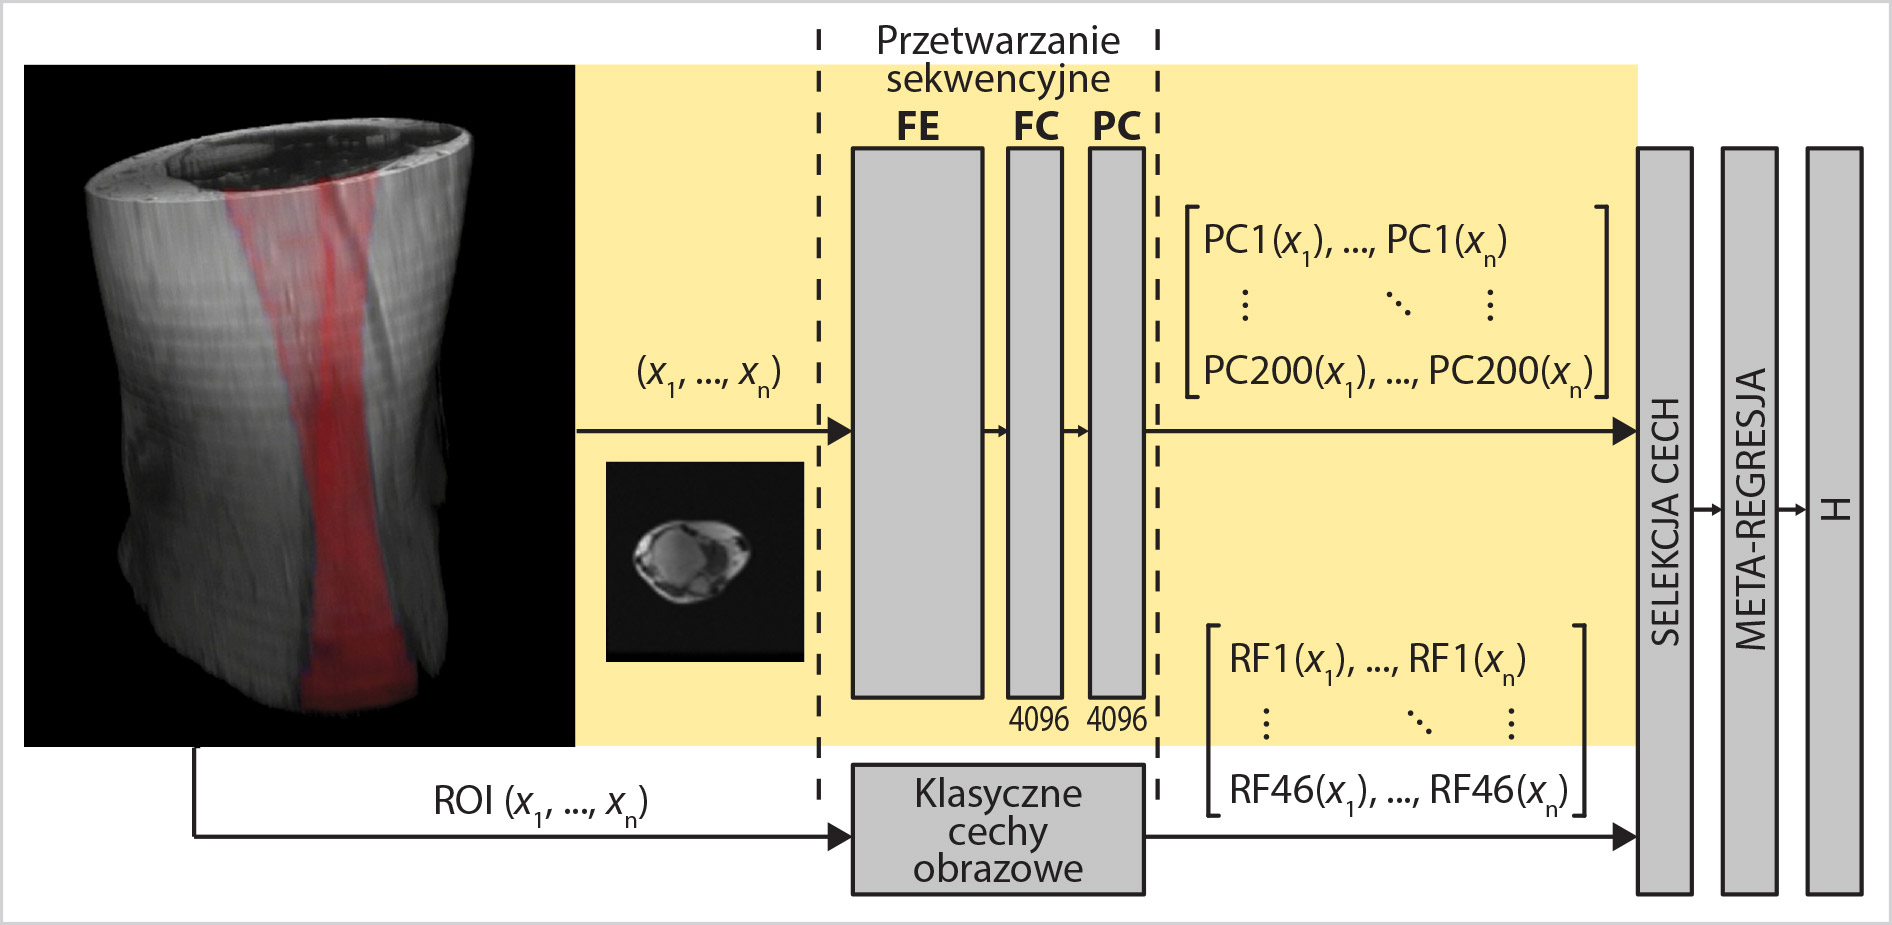
\includegraphics[width=\textwidth]{figures/net.jpg}
	\caption{Schemat automatycznej metody oceny procesu gojenia się ścięgna Achillesa.} \label{fig:net}
\end{figure}
W ogólnym ujęciu, trójwymiarowe badanie RM dzielone jest na pojedyncze przekroje osiowe, które stanowią dane wejściowe do oznaczonej na żółto części opartej o metody głębokiego uczenia się. W tym komponencie dane przetwarzane są przez ekstraktor cech sieci AlexNet (FE), którego parametry wybrano w wyniku eksperymentów. Otrzymane cechy wstępnie grupowane są z wykorzystaniem warstwy gęstej (FC) \linebreak i redukowane z 4096-ciu pojedynczych wyjść aktywacyjnych do 200 czynników głównych (PC).

Równolegle, ROI z każdego z przekrojów stanowi dane wejściowe do obliczeń klasycznych cech obrazowych. Końcowa fuzja realizowana jest z wykorzystaniem meta-regresji i metryki $H$. Takie podejście zapewnia numeryczny opis składający się z pojedynczej wartości dla całego badania RM.

\subsection{Zbiór danych}
\label{seq:zbior-danych}
Dane wykorzystane w tej pracy zostały zebrane w ramach projektu START "Wykorzystanie autologicznych mezenchymalnych komórek macierzystych w procesie regeneracji rekonstruowanego ścięgna Achillesa" finansowanego z konkursu STRATEGMED1 przez Narodowe Centrum Badań i Rozwoju. W ramach projektu, \linebreak do badanej grupy zakwalifikowano 60-ciu pacjentów po całkowitym zerwaniu ścięgna Achillesa i 29-ciu ochotników stanowiących grupę odniesienia. 

Kryteria wykluczające z grupy badanej zostały zdefiniowane tak, aby kwalifikowane osoby nie posiadały wcześniejszej historii urazów ścięgna Achillesa, ani przewlekłych chorób, które mogłyby spowodować degenerację tkanki ścięgnistej. Uwzględniono również warunki odbiegające od normy takie jak: otyłość, ciąża i infekcje. Ostatecznie, w ramach grupy pacjentów znalazło się 49 mężczyzn i 11 kobiet w wieku pomiędzy 24 a 49 lat, ze średnią 36 lat. Wszyscy pacjenci podpisali stosowne zgody wymagane do przeprowadzenia badań.   

52-óch z pośród 60-ciu pacjentów zerwało ścięgna podczas uprawiania sportu. Dokładniej były to: piłka nożna (19), squash/tenis (8), koszykówka (4), bieganie (3), podskoki (2), siatkówka (2) oraz badminton, box, piłka ręczna, fitness, cross-fit, skateboard, rugby i skakanka. Urazy w 31 przypadkach dotyczyły prawego ścięgna, \linebreak a w 29-ciu lewego. Średnia pozycja zerwania umiejscowiona była 57 mm ponad górnym konturem kości piętowej.

W okresie do tygodnia po urazie, pacjenci przeszli zabieg rekonstrukcji wykonany metodą szycia na otwartym ścięgnie (zob. p. \ref{gojenie}). Następnie rozpoczęto rehabilitację trwającą 12 miesięcy, monitorowaną z wykorzystaniem RM i USG. Wykonano również badania biomechaniczne w środkowym i końcowym okresie rehabilitacji, zgodnie z protokołem opisanym w p. \ref{biomechanika}.

Przy akwizycji danych z wykorzystaniem RM posłużono się aparatem GE Signa HDxt 1.5T wyposażonym w cewkę Foot \& Ankle dedykowaną do pomiarów w rejonie dolnej kończyny. Każde z badań RM było wykonane z użyciem 7 sekwencji i łącznie 10 modalności opisanych szczegółowo w p. \ref{RM}:
\begin{enumerate}[noitemsep,nolistsep]
	\item T1 zależne
	\item T2 zależne
	\item PD
	\item T2 mapping
	\item T2$^\ast$ GRE
	\item T2$^\ast$ GRE TE\_MIN
	\item 3D FSPGR
	\begin{itemize}
		\item In Phase Ideal
		\item Out Phase Ideal
		\item Fat Ideal
		\item Water Ideal 
	\end{itemize}
\end{enumerate}

W grupie zdrowych ochotników przeprowadzono pojedyncze badanie, natomiast pacjentów skanowano 10-krotnie w odpowiednio zdefiniowanych odstępach czasowych. Pierwsze badanie odbyło się przed operacją, a następnych 9 odpowiednio \linebreak w tygodniach: 1, 3, 6, 9, 12, 20, 26, 40 i 52 po operacji. W procesie zbierania danych wystąpiły problemy wynikające z braku obecności poszczególnych osób na badaniach lub z niespójności danych. Dlatego finalnie skompletowany zbiór składał się z homogenicznych badań 27 zdrowych ochotników (270 trójwymiarowych skanów RM, w skład których wchodziło wspomniane 10 modalności) oraz 59 badań pacjentów (5900 trójwymiarowych skanów RM z 10-oma modalnościami i 10-oma krokami czasowymi). Przykładowa wizualizacja danych pacjenta i osoby zdrowej znajduje się na Rys. \ref{fig:MRI_sample}. 
\begin{figure}[h!]
	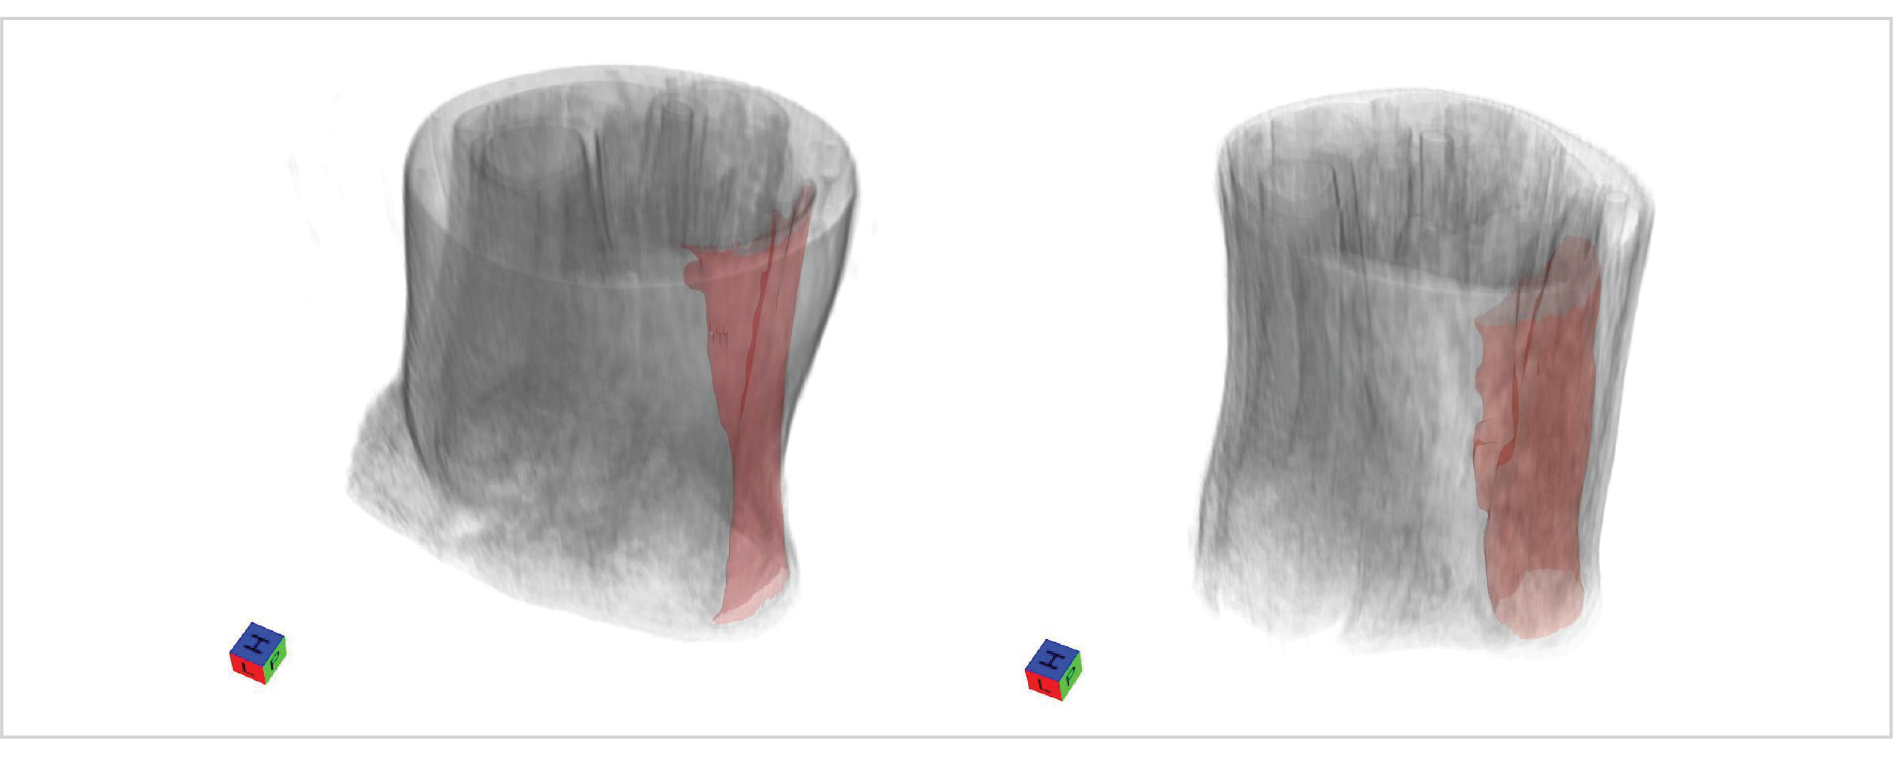
\includegraphics[width=\textwidth]{figures/Data_MRI_sample.jpg}
	\caption{Wizualizacja danych RM w sekwencji PD dla zdrowego (po lewej) i gojącego się (po prawej) ścięgna Achillesa.}
	 \label{fig:MRI_sample}
\end{figure}
Obszar zajmowany przez tkankę ścięgnistą został oznaczony na czerwono. Należy zwrócić uwagę na różnicę w kształcie, która dla zdrowego przykładu jest zgodna z opisem anatomicznym ujętym w p. \ref{anatomia}, natomiast dla przykładu chorego zawiera liczne deformacje. 

Spośród 59-ciu pacjentów zbadanych w ramach projektu START udało się zgromadzić ustrukturyzowany opis radiologiczny dla 48-miu z nich (480 badań). \linebreak W szczególności skompletowano ankietę opisaną w kolejnej podsekcji. Czterech pacjentów zostało losowo wydzielonych na początku eksperymentów jako pacjenci testowi, a pozostali stworzyli grupę pacjentów treningowych.

Zbiory trójwymiarowe posłużyły do opracowania zbiorów dwuwymiarowych składających się z przekrojów. W ten sposób udało się m.in. zwiększyć liczbę próbek wejściowych potrzebnych do szkolenia sieci neuronowych. Dane RM charakteryzują się wysoką anizotropią, a ich rozdzielczość wynosi 512$\times$512$\times$Z, gdzie $Z\in(10:50)$. Wyjątkiem jest sekwencja 3D FSPGR charakteryzująca się niższą anizotropią, jednak większą liczbą artefaktów wynikających z szybkiego czasu akwizycji. Zbiory oparte o RM zostały zatem opracowane w oparciu o przekroje osiowe 512$\times$512. Ważne jest również, że na każdym z tych przekrojów widoczne są elementy ścięgna Achillesa, co nie występuje w danych RM w przypadku przekrojów z pozostałych dwóch płaszczyzn.

Sumaryczna liczba tak uzyskanych próbek dwuwymiarowych wyniosła 11.725 (oznaczonych jako obrazy zdrowego ścięgna) i 138.604 (oznaczonych jako obrazy chorego ścięgna). W zależności od eksperymentów służących do optymalizacji parametrów metody wykorzystano:
\begin{itemize}[noitemsep,nolistsep]
	\item Powiększony zbiór treningowy RM -- zawierający przekroje osiowe ze wszystkich badań pacjentów treningowych, realizowanych wszystkimi sekwencjami. Liczba przekrojów w tym zbiorze została powiększona poprzez zastosowanie transformacji odbicia lustrzanego i, w przypadku chorych przykładów, 10-ciu obrotów w zakresie od -10 do 10 stopni. Finalnie, zbiór zawierał 234.502 przekrojów oznaczonych jako zdrowych i 277.208 oznaczonych jako chorych.
	\item Ograniczony zbiór treningowy RM -- zawierający przekroje osiowe ze zbioru 44-ech pacjentów treningowych jedynie w sekwencji T2$^\ast$ GRE TE\_MIN (18.863 próbek).
	\item Zbiór PCA -- wykorzystywany dalej w pracy do analiz PCA, zawierający próbki z powiększonego zbioru treningowego \linebreak ze wszystkich sekwencji RM dla 10-ciu losowo wybranych pacjentów (44.813).
\end{itemize}

W celu wnioskowania i porównań rezultatów metody posłużono się danymi \linebreak od 4-ech pacjentów testowych, z wykorzystaniem, w zależności od potrzeby, od 1 do 10 modalności RM. Szczegóły dotyczące poszczególnych wyborów znajdują się \linebreak w opisach eksperymentów.


\subsection{Wzorzec odniesienia}
\label{seq:ground-truth}
Do stworzenia wzorca odniesienia, w ramach projektu START, została powołana specjalna grupa robocza składająca się z eksperta radiologa, specjalistów ortopedów i ekspertów od komputerowo wspomaganej diagnostyki. Celem grupy było opracowanie opisu ilościowego odzwierciedlającego elementy, na podstawie których radiolog podejmuje subiektywną opinię. W wyniku prac stworzono zestaw sześciu parametrów oceniany w skali 0--7, opisujący proces gojenia się ścięgna Achillesa widoczny w obrazach RM:

\begin{enumerate}[noitemsep,nolistsep]
	\item Uszkodzenia śródścięgniste (SCT od ang. \textit{Structural Changes within the Tendon}) -- informuje o spójności włókien w obszarze ścięgna. Zawiera się w ROI. Ocena wykonywana zarówno w płaszczyźnie osiowej jak i strzałkowej\footnote{Wykorzystano oś skanowania, z uwagi na techniczne ograniczenia rezonansu -- zwłaszcza anizotropowość obrazów.}. 0 – całkowity brak uszkodzeń, 1 – bardzo małe uszkodzenia. 2 – małe uszkodzenia, 3 – uszkodzenia średniej wielkości , 4 – dość duże uszkodzenia. 5 – duże uszkodzenia, 6 - bardzo duże uszkodzenia, 7 - ekstremalnie duże uszkodzenia.
	\item Pogrubienie ścięgna (TT od ang. \textit{Tendon Thickening} -- najgrubsze miejsce (tj. najdłuższy wymiar) w kierunku strzałkowym widoczny na przekroju osiowym. Zawiera się w ROI. 0 – całkowity brak pogrubienia (3 mm--5 mm), 1 – bardzo małe pogrubienie (6 mm), 2 – małe pogrubienie (9 mm), 3 – średnie pogrubienie (12 mm), 4 –  dość duże pogrubienie (15 mm), 5 duże pogrubienie (18 mm), 6 – bardzo duże pogrubienie (21 mm), 7 – ekstremalnie duże pogrubienie (24 mm).
	\item Ostrość granic ścięgna/rozgraniczenie (STE od ang. \textit{Sharpness of the Tendon Edges}) -- informuje o jakości granicy między tkankami ścięgnistymi i otoczeniem, w szczególności czy brzeg jest fraktalny. Oceniane jest na zewnątrz ścięgna w płaszczyźnie osiowej. 0 – bardzo duża (idealna) ostrość, 1 – duża ostrość, 2 – dość duża ostrość, 3 – średnia ostrość, 4 – mała ostrość, 5 – bardzo mała ostrość, 6 – minimalna ostrość, 7 – całkowicie nieostre.
	\item Obrzęk ścięgna (TE od ang. \textit{Tendon Edema}) -- informuje o anomaliach \linebreak w gromadzeniu się płynów w obszarze ścięgna. Zawiera się w ROI i jest oceniany na przekrojach osiowych. 0 – całkowity brak obrzęku, 1 – bardzo mały obrzęk, 2 – mały obrzęk, 3 – obrzęk średniej wielkości, 4 – dość duży obrzęk, 5 – duży obrzęk, 6 – bardzo duży obrzęk, 7 -- ekstremalnie duży obrzęk.
	\item Jednorodność ścięgna (TU od ang. \textit{Tendon Uniformity}) -- informuje o prawidłowej teksturze poszczególnych przekrojów osiowych i podobieństwie sąsiednich przekrojów mierzonym w płaszczyźnie strzałkowej. Zawiera się w ROI. 0 – całkowity brak niejednorodności (jednorodne), 1 – bardzo małe niejednorodności, 2 – małe niejednorodności, 3 – niejednorodności średniej wielkości, 4 – dość duże niejednorodności, 5 – duże niejednorodności, 6 – bardzo duże niejednorodności, 7 –  ekstremalnie duże niejednorodności. 
	\item Obrzęk tkanek (TisE od ang. \textit{Tissue Edema}) -- informuje o powiększonym przedziale powięziowym ścięgna. 0  – całkowity brak obrzęku, 1 – bardzo mały obrzęk, 2 – mały obrzęk, 3 – obrzęk średniej wielkości, 4 – dość duży obrzęk, 5 – duży obrzęk. 6 – bardzo duży obrzęk, 7 -- ekstremalnie duży obrzęk.
\end{enumerate}

\section{Eksperymenty}
\label{seq:experiments}
W tej sekcji zaprezentowano eksperymenty mające na celu dobór poszczególnych komponentów i parametrów finalnej metody. W pierwszej kolejności zostało opisane badanie dotyczące szkolenia sieci neuronowych, celem wyboru ekstraktora cech dającego możliwość rozróżnienia ścięgien zdrowych od tych po zerwaniu (chorych). Następnie zaprezentowano badanie dotyczące obliczenia wektora cech na wyjściu sieci neuronowej i redukcji jego wymiarowości. W kolejnej części przedstawiono wybór sekwencji RM, stanowiących dane wejściowe do proponowanego w tej pracy algorytmu. Finalnie, w dwóch ostatnich podsekcjach, opisano dobór optymalnego zestawu cech ekstrahowanych z użyciem sieci neuronowej i klasycznych metod przetwarzania obrazów oraz fuzję z wykorzystaniem meta-regresji.  


\subsection{Rozróżnienie ścięgna zdrowego i po zerwaniu}
\label{binaryMRI}
W tym badaniu porównane zostały współczesne architektury sieci neuronowych w zadaniu klasyfikacji binarnej, rozróżniającej obrazy zdrowego od chorego ścięgna. W porównaniu uwzględniono topologie AlexNet (zob. p. \ref{AlexNet}), GoogLeNet Inception-v3 (zob. p. \ref{googlenet}) i ResNet-18 (zob. p. \ref{resnet}). W celu doboru hiperparametrów i optymalizacji parametrów sieci, zastosowano szkolenie z wykorzystaniem kroswalidacji z podziałem na 5 segmentów (zob. p. \ref{sec-overffiting}). W każdym z 5-ciu cykli, 3 segmenty były wykorzystane do treningu, 1 do walidacji i 1 do finalnych testów. Do celów tego badania wykorzystano powiększony zbiór treningowy RM. Wyniki zebrano w Tab. \ref{tab:binary-cross-validation}.
\vspace{10px}
\renewcommand{\arraystretch}{1.2}
\begin{table}[h!]
	\setlength{\tabcolsep}{14pt}
	\centering
	\caption{Wyniki szkolenia sieci neuronowych z wykorzystaniem kroswalidacji z podziałem na 5 segmentów, dla problemu klasyfikacji obrazów zdrowego i chorego ścięgna.}
	\label{tab:binary-cross-validation}
	\begin{tabular}{l | l | l | l | l }
		%\hline
		 & Średnia & Min   & Max   & $\sigma$   \\ \hline \hline
		AlexNet   & 99,19 & 99,15 & 99,24 & 0,04 \\ \hline
		ResNet-18 & 95,98 & 92,78 & 99,04 & 2,5  \\ \hline
		GoogleNet & 99,83 & 99,68 & 99,91 & 0,1  \\ \hline
	\end{tabular}
\end{table}
\renewcommand{\arraystretch}{1}

Dla wszystkich architektur, wyniki dokładności klasyfikacji najlepszych modeli osiągnęły wartość powyżej 99\%. Niemniej jednak, w przypadku architektury ResNet-18, najgorszy model klasyfikował z dokładnością 92,78\%, co przełożyło się również na najgorszy średni wynik równy 95,98\%. Fakt ten może wskazywać na tendencje \linebreak do nadmiernego dopasowywania się architektury ResNet-18. Niższa generalizacja modelu może wynikać z faktu tendencji tej architektury do ekstrakcji cech szczegółowych przez jądra splotu o wymiarze 3$\times$3 lub też niedoboru liczby danych wejściowych w odniesieniu do efektywnej optymalizacji wag splotu.

W kolejnym kroku, dla wszystkich trzech architektur, porównano czasy szkolenia przy zadanym problemie. Na Rys. \ref{fig:training_times} zestawiono łączny czas 5-iu iteracji procesu kroswalidacji.
\begin{figure}[h!]
	\includegraphics[width=\textwidth]{figures/TrainingtimesChart.jpg}
	\caption{Porównanie czasów treningu architektur na dwóch architekturach GPU: Pascal i Volta.}
	\label{fig:training_times}
\end{figure}
Porównano dwie architektury GPU, starszą Pascal P100 i nowszą Volta V100, zaprezentowaną w 2017 roku, charakteryzującą się udoskonalonym, osobnym układem optymalizowanym pod kątem operacji tensorowych realizowanych \linebreak w warstwach konwolucyjnych. Do szkolenia wykorzystano framework Caffe. Można zaobserwować, że wykorzystanie nowszej architektury GPU dało rezultaty około dwukrotnego przyspieszenia czasu szkolenia w przypadku AlexNet i ResNet oraz około 30\% w przypadku GoogLeNet. AlexNet zawiera najmniej warstw konwolucyjnych i optymalizowaną implementację klasyfikatora. Szkolenie tej architektury zajęło mniej niż jedną godzinę na GPU Volta. Dla porównania, sieci z bardziej skomplikowaną topologią tj. ResNet-18 i GoogLeNet, charakteryzują się odpowiednio czasami szkolenia w okolicach 20-stu i 48-miu godzin. 

Na podstawie zestawienia wyników dokładności klasyfikacji z czasami treningu można stwierdzić, że AlexNet i GoogleNet charakteryzują się większą generalizacją, a z tych dwóch modeli, czas szkolenia jest o blisko 47 godzin krótszy dla AlexNet. Dlatego właśnie ekstraktor cech tej architektury został wybrany do realizacji kolejnych eksperymentów. 

Należy również podkreślić, że istnieją sposoby na dalsze poprawienie wyników dokładności wnioskowania. Uzupełniające badanie dotyczące możliwości fuzji sieci AlexNet i ResNet-18 zostało opublikowane przez autora tej pracy w czasopiśmie Acta of Bioengineering and Biomechanics \cite{Kapinski19}. Wyniki mogą być również poprawione poprzez analizę lokalizacji przekrojów w przestrzeni trójwymiarowej, w szczególności poprzez uwzględnienie, że przekroje oddalone od miejsca zerwania bardziej przypominają tkanki zdrowe. Można zatem zastosować np. metody logiki rozmytej lub miękkiej klasyfikacji (zob. \cite{Liu2011}) w celu lepszego określenia przynależności próbek do klas. 

Powyższe podejścia w opinii autora tej pracy miałyby jednak sens tylko w przypadku uzyskania nowych danych, dla których proponowany algorytm uzyskiwałby gorsze rezultaty. Z uwagi na wysokie wyniki dokładności zaprezentowanego podejścia dla wykorzystywanego w tej pracy zbioru, na tym etapie badań autor nie zdecydował się na dalsze usprawnienia kosztem komplikacji algorytmu. Eliminacja wykrytych anomalii i wyników odosobnionych realizowana jest w tej pracy poprzez zastosowanie średniej trymowanej w zaproponowanej metryce $H$ (zob. wzór \ref{ecq:H}).

\subsection{Obliczanie i redukcja wymiarowości wektora cech}

Celem tego eksperymentu jest znalezienie zredukowanego wektora cech $w$ pochodzącego z wyjścia sieci neuronowej. W założeniu ma on zawierać możliwie dużo informacji z oryginalnego zbioru i minimalny wymiar. W tym celu, z oryginalnej architektury AlexNet została wydzielona część ekstraktora cech oraz pierwsza warstwa gęsta (zob. Rys. \ref{AlexNetTopology}). Zabieg ten umożliwił wstępne pogrupowanie cech obrazowych przy jednoczesnym braku ich dywersyfikacji w stopniu jaki robi to pełna sieć. Parametry ekstraktora cech przeniesiono z modelu wybranego w eksperymencie binarnej klasyfikacji. 

Wykorzystując Zbiór PCA (zob. \ref{seq:zbior-danych}) została przeprowadzona analiza czynników głównych (zob. p. \ref{DimReduction}), gdzie pojedynczą obserwację stanowił wektor 4096 aktywacji na wyjściu zmodyfikowanej architektury AlexNet. Porównanie poziomu wariancji zachowywanej przez różną liczbę czynników głównych zebrano w Tab. \ref{PCA-results}.
\vspace{10px}
\renewcommand{\arraystretch}{1.2}
\begin{table}[h!]
 \setlength{\tabcolsep}{12pt}
 \centering
 \caption{Rezultaty PCA dla 1, 10 i 200 pierwszych czynników głównych.}
 \label{PCA-results}
 \begin{tabular}{l|l|l|l}
 
 & PC1 & PC1--PC10 & PC1--PC200 \\ \hline \hline
 Udział wyjaśnionej wariancji & 50,2\% & 90,8\%   & 98,8\% \\ \hline 
 \end{tabular}
 \end{table}
\renewcommand{\arraystretch}{1}

Analiza umożliwiła redukcję wymiarowości i rozróżnienie między obserwacjami w poszczególnych krokach czasowych. Wyjścia po transformacji PCA nazywane \linebreak są dalej w pracy \textit{cechami DL}. Można zaobserwować, że 4096 wartości zredukowanych do jednej cechy DL zachowuje ponad 50\% poziomu wariancji. Odpowiednio 10 cech DL zapewnia poziom powyżej 90\%, a 200 poziom bliski 99\%. 

W kolejnym kroku zwizualizowano uśrednione wartości PC1 dla wyników wszystkich pacjentów ze zbioru PCA w kolejnych tygodniach rehabilitacji (zob. Rys. \ref{fig:H}).

\begin{figure}[h!]
	\centering
	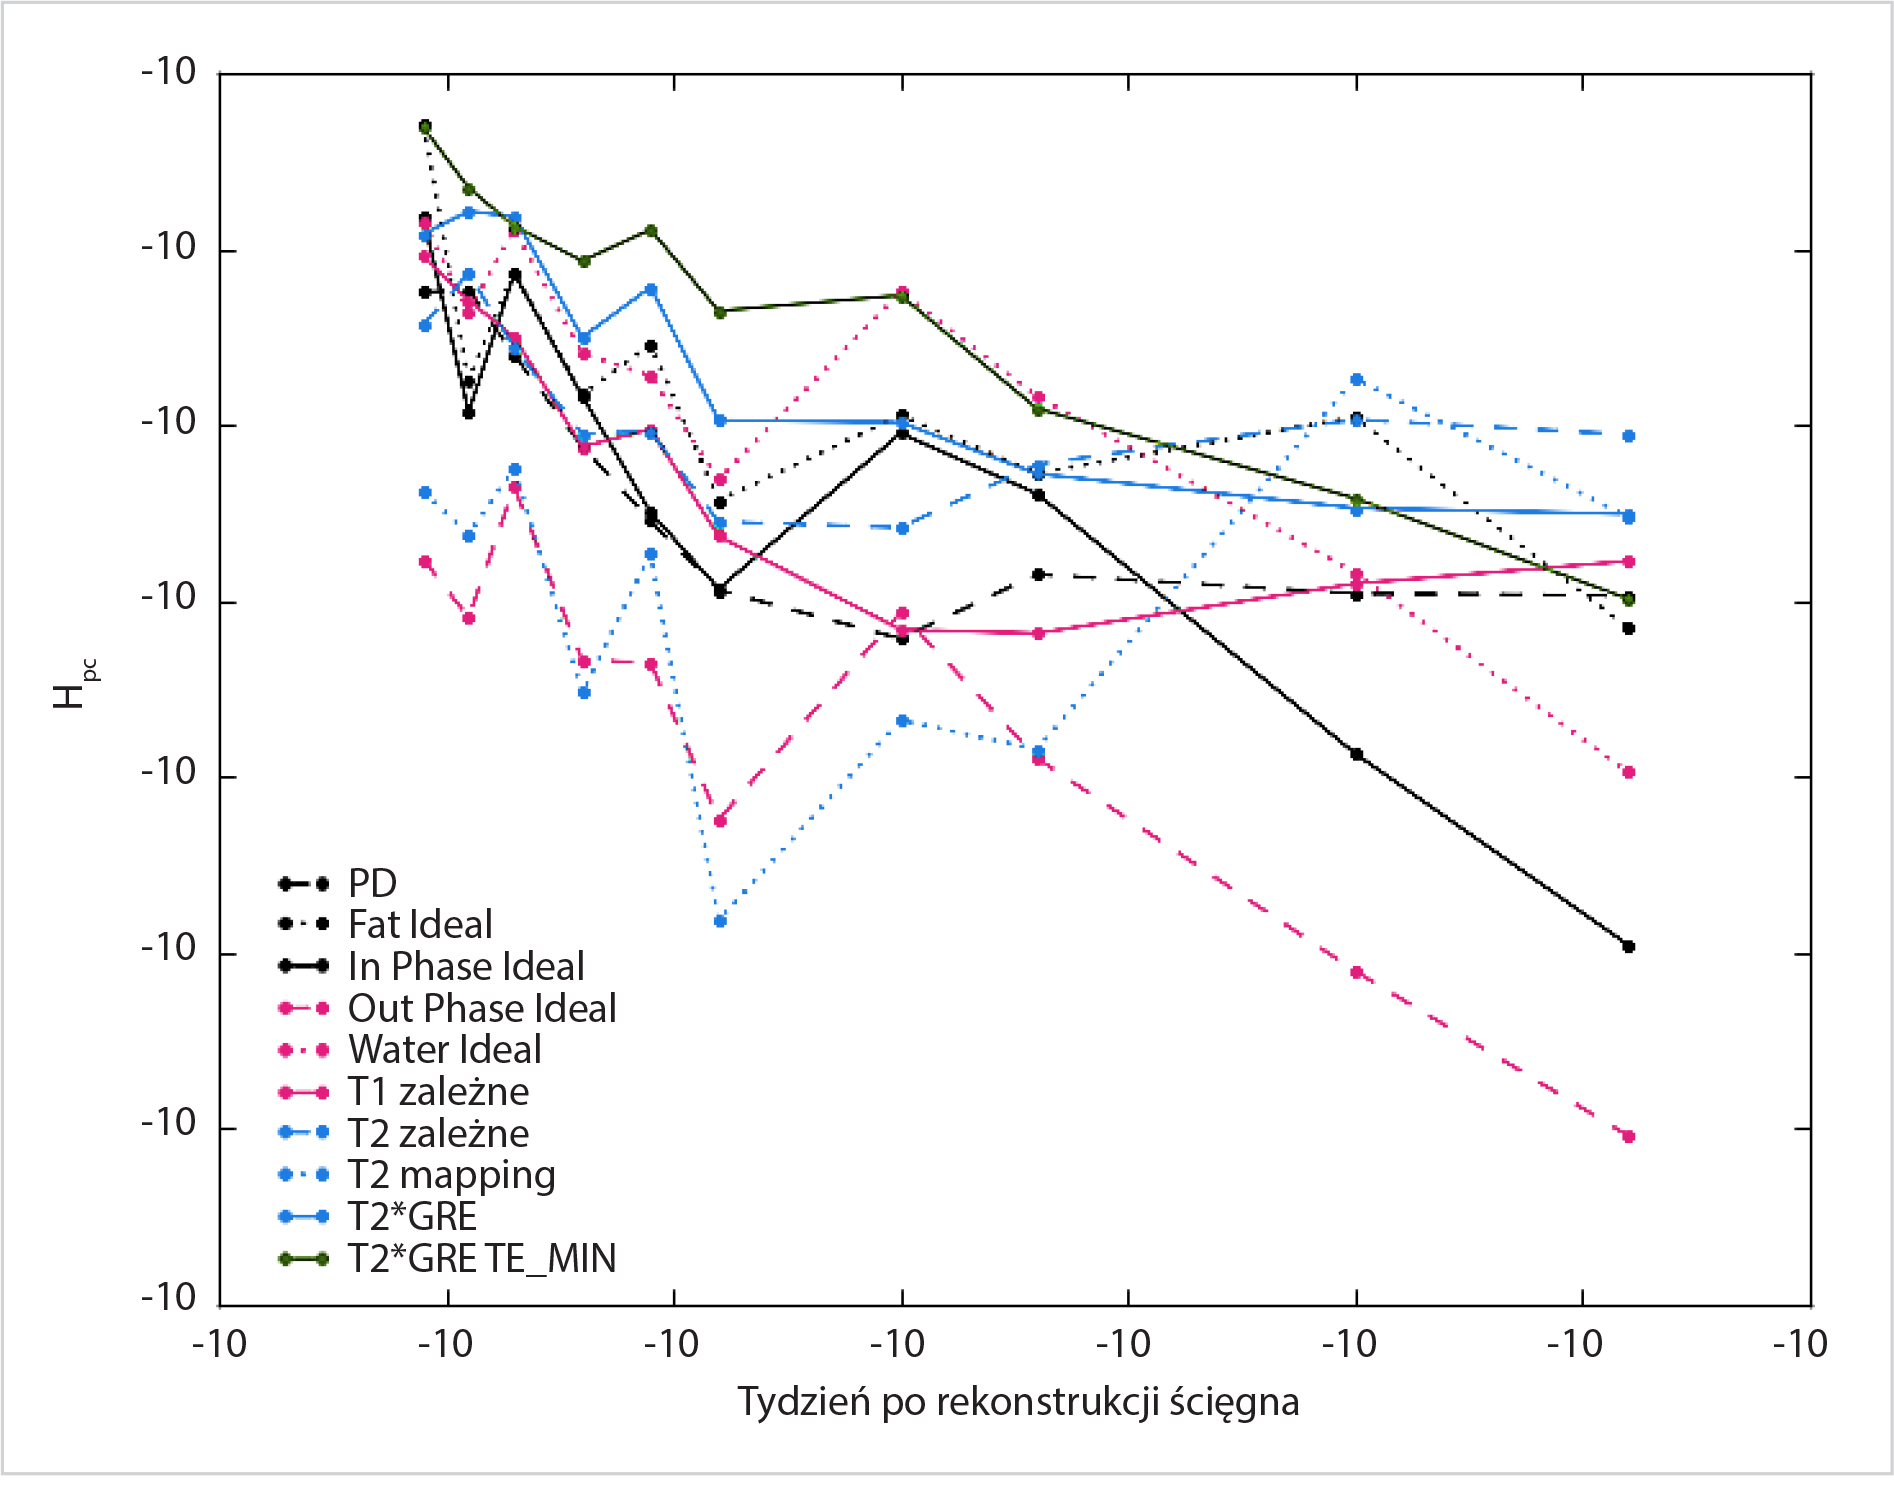
\includegraphics[width=1\textwidth]{figures/H_PC1.jpg}
	\caption{Porównanie krzywych dla 10 modalności RM reprezentujących średnią $H_{PC}$ z 10 pacjentów.}\label{fig:H}
\end{figure}
Oddzielnie przedstawiono wykresy uzyskanych krzywych dla wszystkich użytych w tej pracy sekwencji i modalności RM. W celu uzyskania pojedynczej wartości opisującej badanie RM wykorzystano ponownie średnią trymowaną:

\begin{equation}
\label{ecq:HPC}
H_{PC} = TM(PC1(x_1), PC1(x_2),..., PC1(x_n)).
\end{equation}

Wizualizacja umożliwia lepsze zrozumienie informacji zachowywanej przez użytą transformację PCA. Oprócz sekwencji T2 mapping, wszystkie pozostałe pokazują malejący trend rozumiany jako ujemna różnica pomiędzy wartością końcową i początkową okresu rehabilitacji. Odmienny trend T2 mapping może być spowodowany faktem, że dla tej sekwencji dane były zbierane we wszystkich 8-miu poziomach sygnału T2. W związku z tym, w obrazach pojawiają się próbki silnie zaszumione \linebreak i zniekształcone. Dopiero głębsza analiza związana np. z wyliczeniami na podstawie aproksymacji wartości poziomów T2 może skutkować efektywnym wykorzystaniem T2 mapping do oceny zadanego w tej pracy problemu (zob. \cite{Regulski2017}). 

W pozostałych przypadkach zaobserwować można istotne z punktu widzenia oceny gojenia etapy. Na początku procesu zmiany w badaniach obrazowych są bardzo wyraźne, co uwidocznione jest w postaci charakterystycznych minimów i maksimów lokalnych występujących do 20-tego tygodnia, gdzie wprowadzane są obciążanie nogi i kolejny etap rehabilitacji. Po tym okresie proces gojenia jest mniej dynamiczny. Ten ogólny schemat zaburzony jest przez fluktuacje zależne od indywidualnych cech pacjenta oraz czynników takich jak przestrzeganie zaleceń rehabilitacji, diety i aktywności pacjenta. 

Podsumowując, użyta transformacja pozwala na uzyskanie zredukowanego wektora cech DL, zawierającego od 1 do 200-stu wartości i zachowującego 50,2--98,8\% informacji. Średnie trendy tak otrzymywanych wartości wskazują również na możliwość wnioskowania co do procesu gojenia się ścięgna.  


\subsection{Wybór sekwencji rezonansu magnetycznego}
\label{seq:protocol_selection}
Z uwagi na opisany w p. \ref{RM} tor akwizycji danych RM, zwiększanie liczby sekwencji odbywa się kosztem wydłużenia czasu badania pacjenta. W skrajnym przypadku, takim jak pozyskanie wszystkich 10-ciu omawianych sekwencji, czas ten w nowoczesnych systemach wynosi około jednej godziny, co stanowi praktyczne ograniczenie opracowywanej metody. Dlatego celem tego eksperymentu jest wybór protokołu zawierającego minimalną liczbę sekwencji, umożliwiających przy użyciu opracowywanej metody skuteczną ocenę procesu gojenia. Prace podzielono na dwa etapy: analizę wizualną i ilościową.

\subsubsection{Analiza wizualna} W ramach wstępnej analizy, wartości danych ze wszystkich sekwencji i modalności zebranych od pacjentów zostały zakumulowane w postaci  histogramów i przedstawione na Rys. \ref{fig:Hists}.
\begin{figure}[]
	\centering
	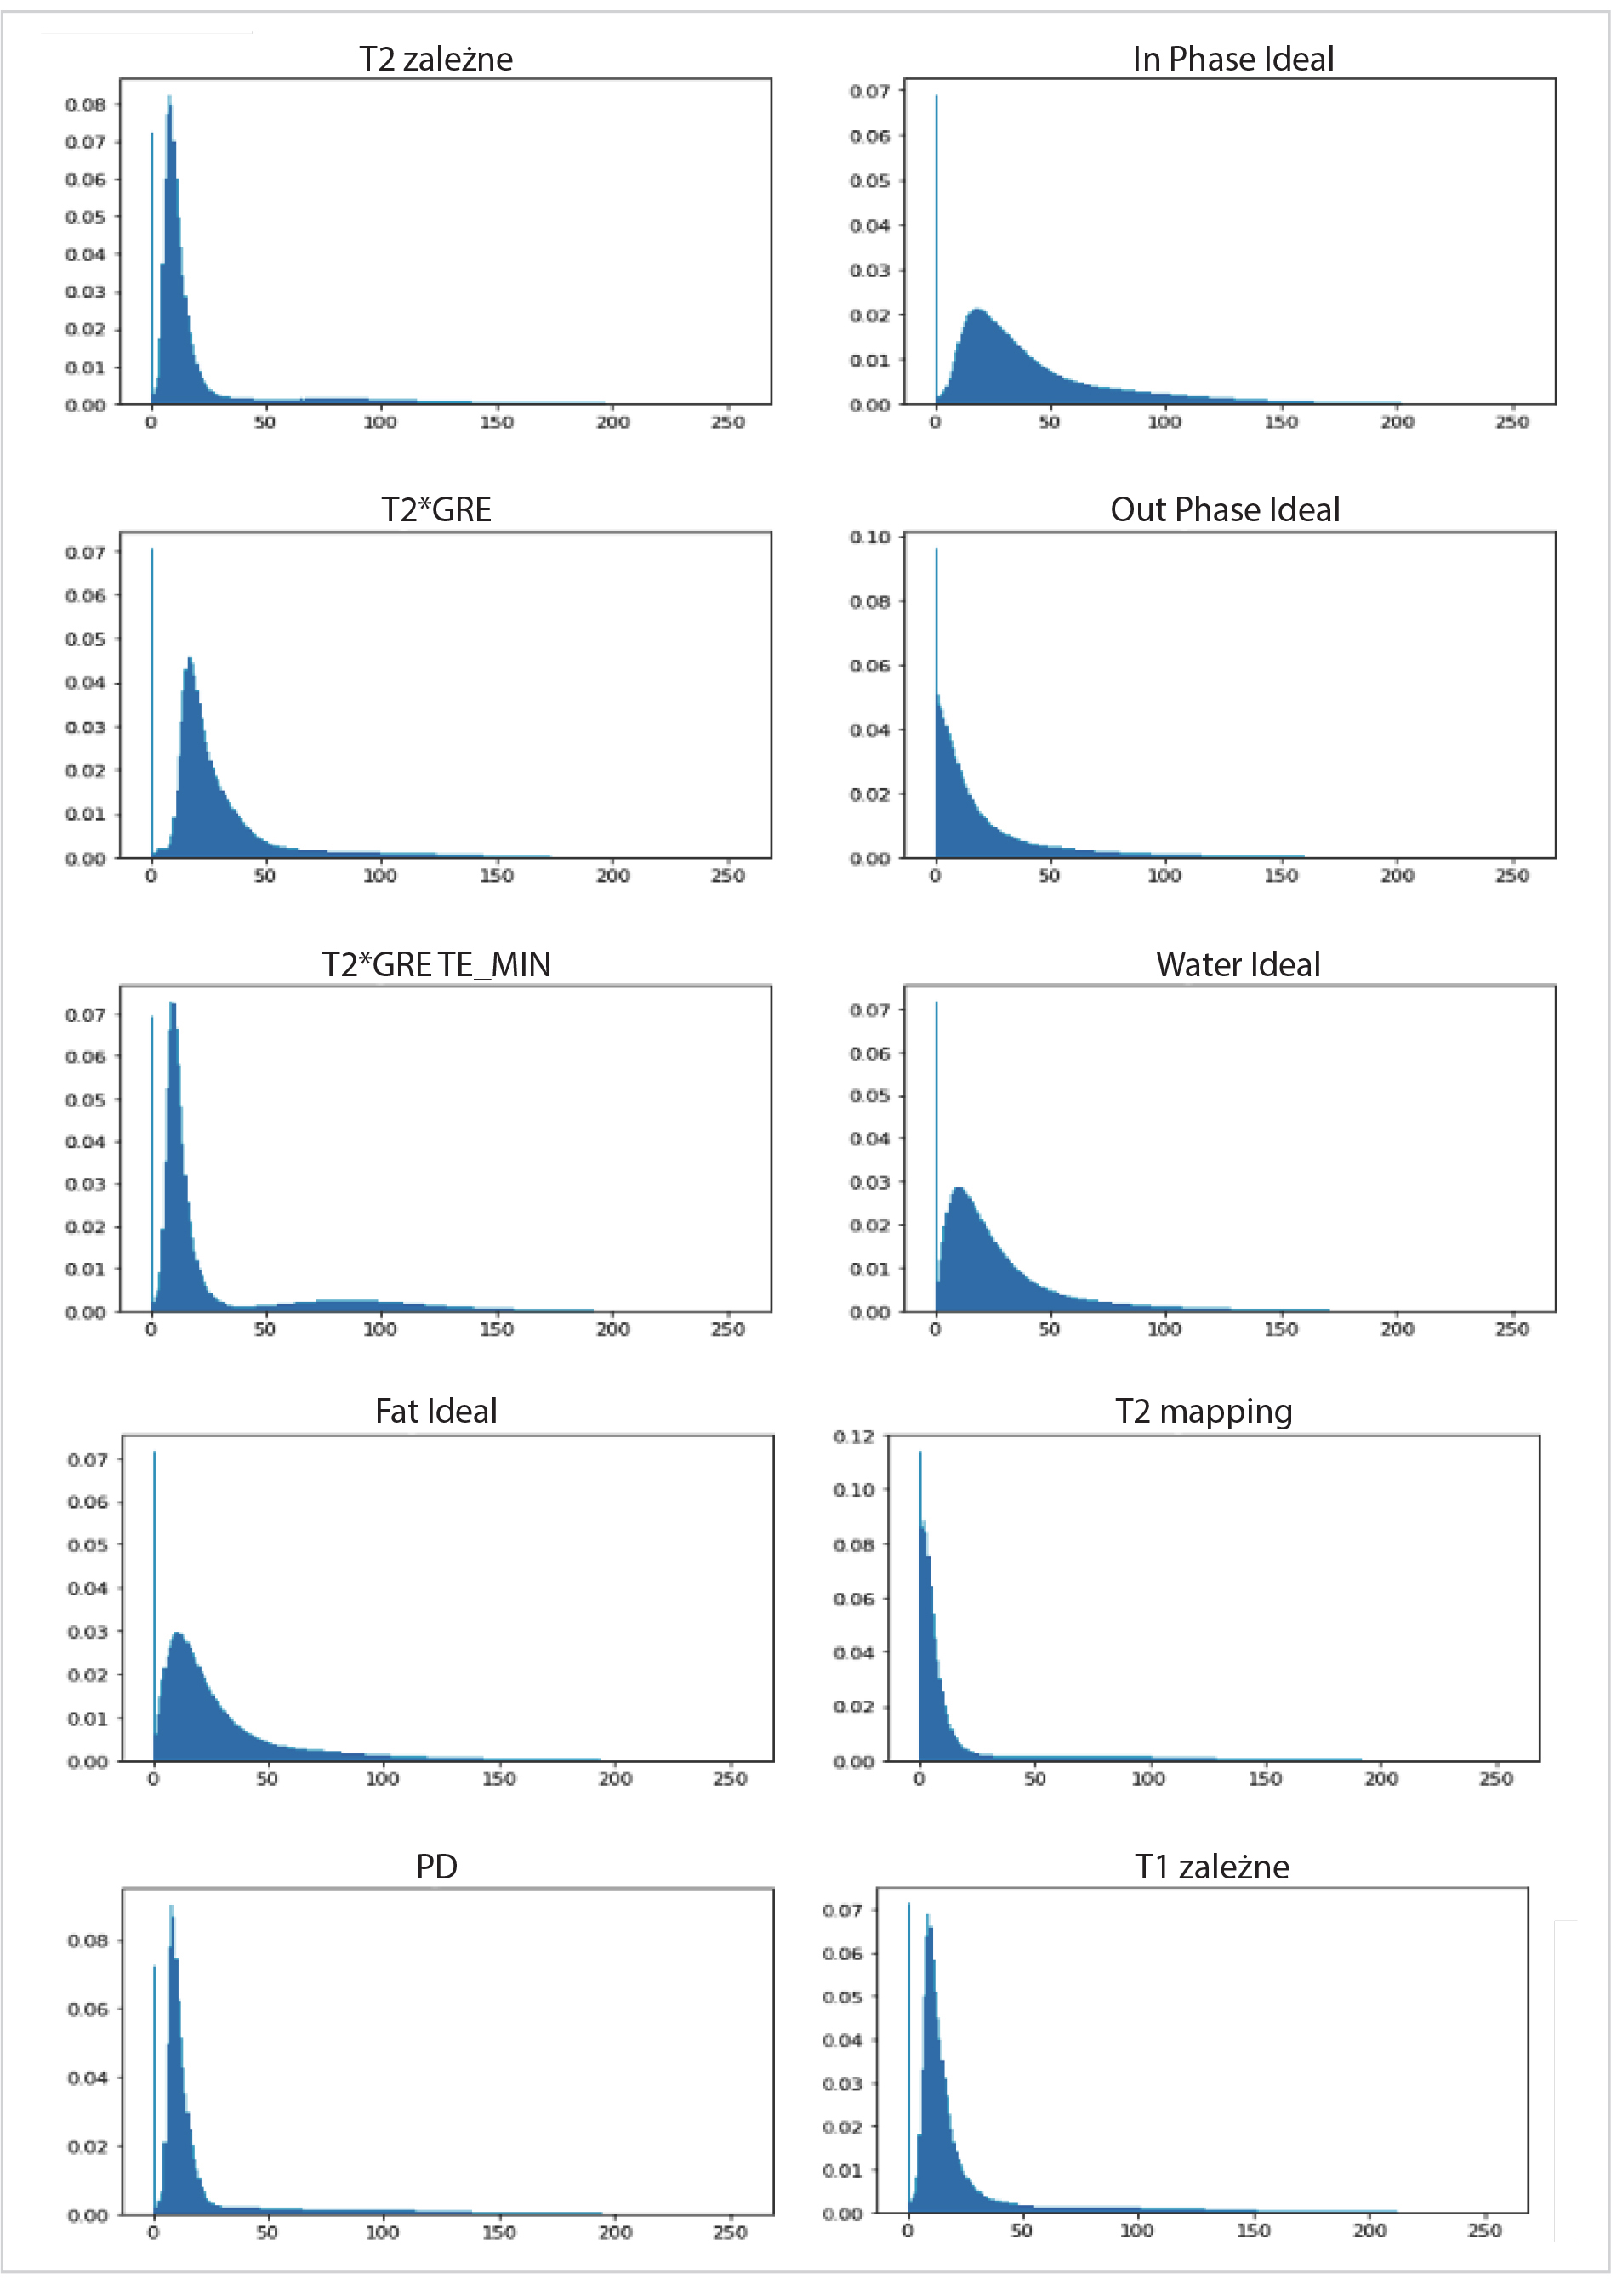
\includegraphics[width=1\textwidth]{figures/Hists.jpg}
	\caption{Znormalizowane histogramy dla 10-ciu sekwencji RM.}\label{fig:Hists}
\end{figure}
Dane zostały przeskalowane do zakresu $<$0; 255$>$ i zmodyfikowane do porównań tak, aby wartość całki Riemanna była równa 1.

Widoczne we wszystkich przypadkach maksima globalne w zerze są naturalnie wynikiem tła, które stanowi powietrze. Analizując pozostałe wartości można wyróżnić następujące 3 grupy:

\begin{enumerate}[noitemsep,nolistsep]
	\item Bez maksimum lokalnego -- sekwencja T2 mapping i modalność Out Phase Ideal. W pierwszym przypadku jest to konsekwencja, wspomnianego już w poprzednim eksperymencie, występowania danych ze wszystkich 8-miu próbek sekwencji, czyli również tych mierzonych przy prawie zerowym sygnale T2, silnie zaszumionym, z licznymi wartościami bliskimi zeru. W drugim przypadku, na granicach wody i tłuszczu, występuje często silne rozmycie (tzw. \textit{artefakt czarnego atramentu}), co również zwiększa liczbę wartości bliskich zeru.
	\item Z jednym maksimum lokalnym -- pozostałe modalności 3D FSPGR oraz sekwencje: PD, T1 zależne, T2 zależne, T2$^\ast$ GRE. Przypadek najczęściej występujący. Wartości sygnału zależą od tkanek dominujących w obrazowanym elemencie.
	\item Z dwoma maksimami lokalnymi -- sekwencja T2$^\ast$ GRE TE\_MIN. Jako jedyna posiada drugie maksimum lokalne, co może wskazywać na zwiększoną czułość na wzorce zawarte w danych.  
	
\end{enumerate}
%dlaczego wyrzucamy 3DFSPGR?
Na podstawie powyższej analizy, z uwagi na możliwość występowania wysokiego szumu w sygnale oraz artefaktów, można wyłączyć z dalszych badań pierwszą grupę sekwencji. 

Zdecydowanie wyróżniająca się sekwencją jest T2$^\ast$ GRE TE\_MIN. W celu lepszego zrozumienia istotności różnic występujących na Rys. \ref{fig:protocol_comp} zestawiono przykład rekonstrukcji danych z wykorzystaniem sekwencji z obu analizowanych dalej grup (wyłączono sekwencję 3DFSPGR, której modalności podzieliły się pomiędzy grupy 1 i 2 i która we wstępnych badaniach charakteryzowała się dużym zaszumieniem). 

 \begin{figure}[h]
 	\centering
 	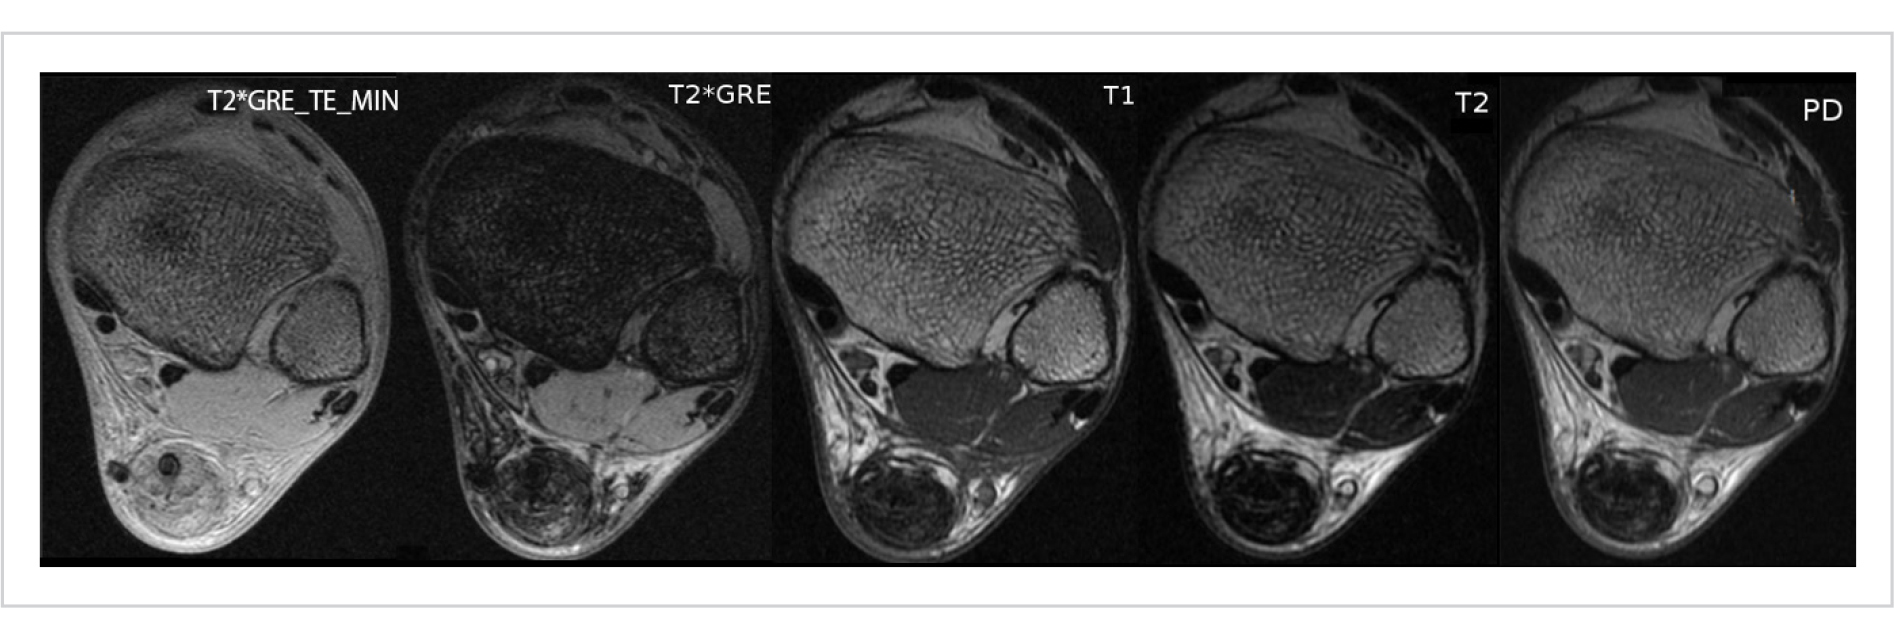
\includegraphics[width=1\textwidth]{figures/Protocol_comparison.jpg}
 	\caption{Porównanie sekwencji RM ilustrujących proces gojenia się ścięgna Achillesa w 12-tym tygodniu po rekonstrukcji.}\label{fig:protocol_comp}
 \end{figure}

Istotna różnica w rekonstruowanych obrazach pochodzi z poziomów odcieni szarości w obszarze ścięgna. Obrazy w dwunastym tygodniu procesu gojenia się, rekonstruowane przy pomocy sekwencji z grupy 2, charakteryzują się wartościami w obszarze ścięgna bliskimi zeru. Jedynie na obrazach rekonstruowanych z wykorzystaniem danych z T2$^\ast$ GRE TE\_MIN obszar ścięgna jest jaśniejszy. 

Na Rys. \ref{fig:T2comp} przedstawiono próbki T2$^\ast$ GRE TE\_MIN zrekonstruowane w kolejnych krokach czasowych.
\begin{figure}[h]
	\centering
	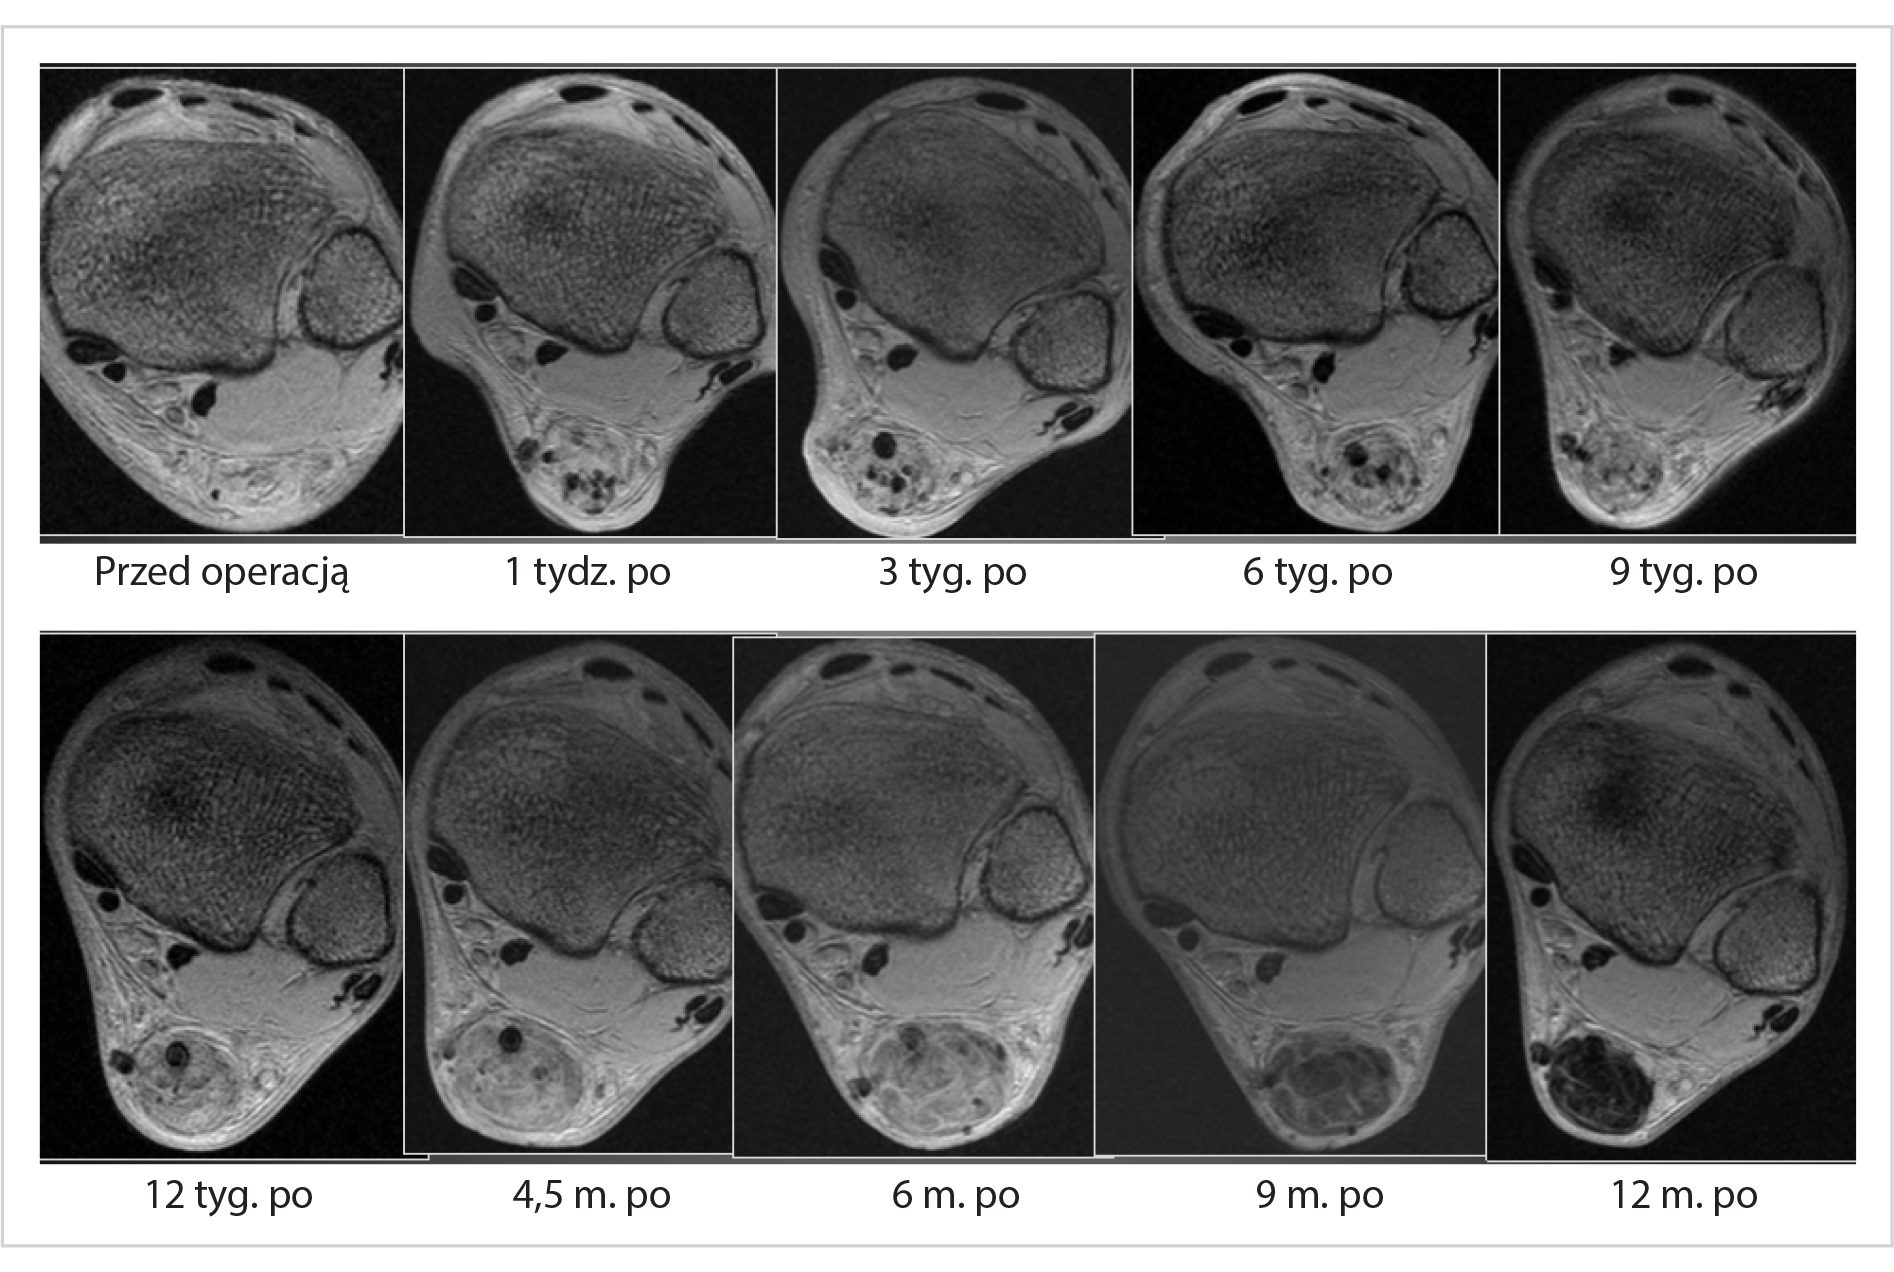
\includegraphics[width=1\textwidth]{figures/T2gremin.jpg}
	\caption{Proces gojenia się ścięgna Achillesa widoczny w obrazach zrekonstruowanych na podstawie danych z sekwencji T2$^\ast$ GRE TE\_MIN.}\label{fig:T2comp}
\end{figure}
Analiza wizualna wskazuje, że różnice w odcieniach szarości mogą wspomóc radiologów w skutecznej interpretacji stopnia wygojenia się tkanek ścięgnistych. Wartości w obszarze ścięgna są jasne na początku i ciemnieją z czasem. 

W sekwencji T2$^\ast$ GRE TE\_MIN, czas TE jest bardzo krótki. W pozostałych sekwencjach wykorzystanych w tej pracy TE $\gg$ T2$^\ast$. Z uwagi na cechy mierzonej tkanki, generowany sygnał ma tendencję do szybkiego zaniku. W T2$^\ast$ GRE TE\_MIN jest on zatem mierzony przed tym faktem, a nie przy wartościach bliskich zeru. \linebreak Na przestrzeni całego procesu gojenia się ścięgna, zmiany uwidaczniają się w postaci silnie rozróżnialnych odcieni szarości w obszarze ścięgna, co z kolei jest również wartościową informacją z uwagi na zastosowane w tej pracy metody sztucznej inteligencji i przetwarzania obrazów. Powyższe obserwacje i wnioski zostały dalej wykorzystane w analizie ilościowej.

\subsubsection{Analiza ilościowa} W ramach tego badania porównano ilościowo wyniki automatycznej oceny procesu gojenia się ścięgna Achillesa przy użyciu danych: (1) tylko z sekwencji \linebreak T2$^\ast$ GRE TE\_MIN; (2) danych z sekwencji T2$^\ast$ GRE TE\_MIN oraz PD i T2$^\ast$ GRE. 
Wybierając sekwencję T2$^\ast$ GRE TE\_MIN kierowano się wynikami analizy wizualnej, natomiast dobór pozostałych dwóch sekwencji, poza analizą wizualną i wiedzą dziedzinową, był umotywowany oceną stopnia korelacji zaprezentowaną w Tab. \ref{tab:inter-protocol-corr}, gdzie zestawiono sekwencje z grupy (2) bez 3DFSPGR.
\vspace{10px}
\renewcommand{\arraystretch}{1.2}
\begin{table}[h]
	\centering
	\setlength{\tabcolsep}{12pt}
	\caption{Korelacja sekwencji PD, T1, T2 i T2$^\ast$ GRE MRI. Wyniki oznaczone pogrubieniem są istotne statystycznie z $p$ $<$ 0,01.}
	\label{tab:inter-protocol-corr}
	\begin{tabular}{l||c|c|c|c}
		%\hline
		& PD & T1 & T2 & T2$^\ast$GRE \\ \hline \hline
		PD & 1,00 & \textbf{0,96} & \textbf{0,90} & \textbf{0,89} \\ \hline
		T1 & \textbf{0,96} & 1,00 & \textbf{0,85} & \textbf{0,92} \\ \hline
		T2 & \textbf{0,90} & \textbf{0,85} & 1,00 & 0,71 \\ \hline
		T2$^\ast$GRE & \textbf{0,89} & \textbf{0,92} & 0,71 & 1,00  %\hline
	\end{tabular}
	%\vspace{-0.5cm}
\end{table} 
\renewcommand{\arraystretch}{1}

Do obliczeń korelacji wybrano wektor cech DL zredukowany do pojedynczej wartości niosącej ponad 50\% informacji, zagregowany dla badania z wykorzystaniem metryki $H_{PC}$ (zob. wzór \ref{ecq:HPC}). Uwzględniając wyniki istotne statystycznie, wśród najbardziej skorelowanych sekwencji znalazły się T1 i PD. PD najmniej koreluje \linebreak z T2$^\ast$GRE, natomiast T1 z sekwencją T2. 

W kolejnym kroku wykorzystano tę informację sprawdzając, w odniesieniu \linebreak do wybranej w analizie wizualnej sekwencji T2$^\ast$ GRE TE\_MIN, czy wnioskowanie co do procesu gojenia, na podstawie cech DL ulega polepszeniu z wykorzystaniem większej liczby różnorodnych sekwencji. 

Wykorzystano ponownie zredukowaną przestrzeń cech DL (tym razem 1--10 czynników głównych) i wykonano szereg obliczeń stopnia gojenia się ścięgna stosując poniższą metrykę: 

\begin{equation}
H_{reg} = \alpha + \sum_{i=1}^{3}\beta_{i}X_{i} + \sum_{i=1}^{3}\gamma_{i}X_{i}^{2} +
\sum_{\substack{i, j = 1\\ i < j}}^{3}\lambda_{i,j}X_{i}X_{j}
\end{equation}

gdzie $X_i = TM(PC_n(x_1), PC_n(x_2),..., PC_n(x_n))_{i}$ to kolejne predyktory odpowiadające próbkom z trzech wykorzystywanych w eksperymencie sekwencji, $TM$ \linebreak to średnia trymowana z marginesami 2,5\%, $PC_n(x_k)$ to $n$-ty czynnik główny otrzymany przy wnioskowaniu sieci dla przekroju osiowego $x_k$, a $k$ jest indeksem przekroju danej sekwencji w trójwymiarowym badaniu RM.

W szczególności, wyliczono różne modele regresji poczynając odpowiednio od liniowej, gdzie ($\gamma_{i}=0, \lambda_{i}=0$), przez nieliniową stopnia drugiego -- $model\_poly$ ($\lambda_{i}=0$) oraz z kombinacją czynników -- $model\_c\_poly$. W przypadku liniowym wykorzystano 1--10 czynników głównych -- odpowiednio $model\_PC[1-10]$. Natomiast w przypadku nieliniowym wykorzystano tylko dwa pierwsze czynniki, ograniczając tym samym efekt nadmiernego dopasowania się modelu. Powyższe modele funkcjonujące w oparciu o trzy sekwencje (tj. T2$^\ast$ GRE TE\_MIN, PD i T2$^\ast$ GRE) zestawiono z modelem liniowej regresji wytrenowanym jedynie na danych z T2$^\ast$ GRE TE\_MIN ($Baseline$). 

Do obliczenia współczynników regresji zastosowano zbiór pacjentów treningowych. Natomiast w celach porównań, zestawiono wyniki dla pacjentów testowych. \linebreak W szczególności, wyliczono metryki średniego błędu absolutnego (MAE), maksymalnego błędu absolutnego (MAX-AE) i średniej korelacji obliczonej z wykorzystaniem transformacji Z-Fishera (Corr). Wybór metryk związanych z błędami absolutnymi był podyktowany faktem, iż skala liniowa okazała się w toku eksperymentów bardziej intuicyjna dla lekarzy i radiologów, a zatem bardziej utylitarna w procesie komunikowania wyników. Rezultaty znajdują się w Tab. \ref{tab:H_testset}.
\renewcommand{\arraystretch}{1.2}
\begin{table}[h!]
	\caption{Porównanie wnioskowania dla różnych modeli regresji wytrenowanych w oparciu o dane z 3-ech sekwencji RM, z modelem liniowej regresji wytrenowanym w oparciu o jedną sekwencję RM. Najlepsze wyniki oznaczono pogrubieniem i dodatkowo, w przypadku istotnej statystycznie poprawy z $p$ $<$ 0,05 liczonych średnich, oznaczono kolorem czerwonym.}
	\scriptsize
	\begin{center}
		\begin{tabular}{lc||c|c|c|c|c|c}
			\textbf{Model} & & \textbf{SCT} & \textbf{TT} & \textbf{STE} & \textbf{TE} & \textbf{TU} & \textbf{TisE}\\ 
			
			\hline \hline
			model\_PC1 & MAE & 1,26 $\pm$ 0,07 & \textcolor{red}{\textbf{0,71}} $\pm$ 0,02 & \textbf{0,7} $\pm$ 0,02 & 0,97 $\pm$ 0,04 & 0,92 $\pm$ 0,04 & 0,99 $\pm$ 0,04\\
			&MAX-AE &3,53&2,49&1,91&\textbf{2,34}&2,2&2,47\\
			&Corr &0,58&0,47&-0,07&0,60&\textbf{0,56}&0,58\\
			
			\hline
			model\_PC1\_2 & MAE & 1,28 $\pm$ 0,07 & 0,74 $\pm$ 0,02 & 0,71 $\pm$ 0,03 & 0,98 $\pm$ 0,04 & 0,94 $\pm$ 0,05 & 1,02$\pm$ 0,04\\
			&MAX-AE &3,64&2,56&1,94&2,98&2,35&2,9\\
			&Corr &0,53&0,30&0,02&0,51&0,41&0,60\\
			
			\hline
			model\_PC1\_3&MAE & 1,43 $\pm$ 0,09 & 0,71 $\pm$ 0,02 & 0,73 $\pm$ 0,03 & 1,02 $\pm$ 0,05 & 1,05 $\pm$ 0,05 & 1,07 $\pm$ 0,06\\
			&MAX-AE &3,99&2,49&1,98&3,2&2,96&3,02\\
			&Corr &0,48&0,36&0,03&0,50&0,29&0,62\\
			
			\hline
			model\_PC1\_4&MAE & 1,39 $\pm$ 0,08 & 0,72 $\pm$ 0,01 & 0,8 $\pm$ 0,02 & 1,01 $\pm$ 0,04 & 1,02 $\pm$ 0,05 & 1,06 $\pm$ 0,05\\
			&MAX-AE &3,56&\textbf{2,4}&2,17&3,2&2,61&3,13\\
			&Corr &0,54&0,37&0,17&0,52&0,38&\textbf{0,68}\\
			
			\hline
			model\_PC1\_5&MAE & 1,35$\pm$ 0,07 & 0,79$\pm$0,01 &0,8$\pm$0,04 &0,99$\pm$0,04 &1,01$\pm$0,04 &1,1$\pm$0,04\\
			&MAX-AE &3,45&2,69&2,39&3,21&2,55&2,88\\
			&Corr &0,49&0,31&0,22&0,52&0,30&0,60\\
			
			\hline
			model\_PC1\_6&MAE & 1,32$\pm$0,07 & 0,78$\pm$0,01 &0,8$\pm$0,04& 0,97$\pm$0,05 & 0,98$\pm$0,04 &1,11$\pm$0,04\\
			&MAX-AE &\textbf{3,3}&2,64&2,21&3,12&2,6&2,8\\
			&Corr &0,53&0,33&0,21&0,56&0,38&0,56\\
			
			\hline
			model\_PC1\_7&MAE &$1,33\pm{0,07}$&$0,78\pm{0,01}$&$0,82\pm{0,04}$&$1,03\pm{0,05}$&$0,99\pm{0,04}$&$1,14\pm{0,05}$\\
			&MAX-AE &3,34&2,75&2,41&3,17&2,63&2,69\\
			&Corr &0,53&0,33&0,21&0,54&0,30&0,57\\
			
			\hline
			model\_PC1\_8&MAE & 1,35$\pm$0,07 & 0,77$\pm$0,01& 0,81$\pm$0,04&1,02$\pm$0,05& 0,99$\pm$0,05 & 1,14$\pm$0,05\\
			&MAX-AE &3,41&2,58&2,47&3,13&2,65&2,75\\
			&Corr &0,54&0,37&0,19&0,53&0,25&0,55\\
			
			\hline
			model\_PC1\_9&MAE & 1,38$\pm$0,07 & 0,74$\pm$0,01 & 0,76$\pm$0,05 & 1,03$\pm$0,05 & 1,02$\pm$0,05 & 1,12$\pm$0,04\\
			&MAX-AE &3,49&2,57&2,45&2,9&2,7&2,67\\
			&Corr &0,52&0,40&\textbf{0,25}&0,55&0,30&0,58\\
			
			\hline
			model\_PC1\_10&MAE & 1,37$\pm$0,07 & 0,74$\pm$0,02 & 0,76$\pm$0,04 & 1,04$\pm$0,04 & 1,03$\pm$ 0,05& 1,11$\pm$0,05\\
			&MAX-AE &3,46&2,42&2,52&2,92&2,67&2,68\\
			&Corr &0,50&0,38&0,24&0,54&0,29&0,59\\
			
			\hline
			model\_poly&MAE & 1,27$\pm$ 0,07 & 0,74$\pm$0,01 & 0,71$\pm$0,03 & \textcolor{red}{\textbf{0,93}}$\pm$0,04 & 0,95$\pm$0,05 & 1,03$\pm$0,04\\
			&MAX-AE &3,62&2,6&1,96&2,83&2,29&2,87\\
			&Corr &0,53&0,34&0,11&\textbf{0,61}&0,37&0,58\\
			
			\hline
			model\_c\_poly&MAE & 1,3$\pm$0,07 & 0,75$\pm$0,01 & 0,78$\pm$0,04 & \textcolor{red}{\textbf{0,93}}$\pm$0,04 & 1,01$\pm$0,06 & 1,06$\pm$0,05 \\
			&MAX-AE &3,64&2,7&2,01&2,83&3,36&2,86\\
			&Corr &0,53&0,45&0,12&0,58&0,15&0,57\\
			\hline 
			
			Baseline& MAE & \textbf{1,24}$\pm$0,08 & 0,82$\pm$0,04 & 0,75$\pm$0,04 & 1,06$\pm$0,05 & \textbf{0,90}$\pm$0,04 & \textbf{0,96}$\pm$0,05 \\
			&MAX-AE & 3,54 & 2,46 & \textbf{1,82} & 2,70 & \textbf{2,13} & \textbf{2,18}\\
			&Corr   & \textbf{0,61} & \textcolor{red}{\textbf{0,64}} &-0,08 & 0,55 & 0,55 & 0,65\\
			\hline
		\end{tabular}
	\end{center}
	\label{tab:H_testset}
\end{table}
\renewcommand{\arraystretch}{1}

Z wykorzystaniem dodatkowych sekwencji udało się uzyskać poprawę istotną statystycznie z $p$ $<$ 0,05 w przypadku MAE dla parametrów TT i TE. W przypadku TT dodanie sekwencji skutkowało natomiast istotnie statystycznym pogorszeniem Corr. Model prostej liniowej regresji wykorzystujący jedynie informacje z sekwencji T2$^\ast$ GRE TE\_MIN ponadto osiągnął najlepsze rezultaty w największej liczbie błędów MAX-AE tj. 3. Można zatem wnioskować, że dodawanie sekwencji jako danych wejściowych i komplikacje modelu skutkują nadmiernym dopasowaniem oraz po za opisanymi wyjątkami nie polepszają jakości automatycznej oceny. Należy również podkreślić, że akwizycja samej sekwencji T2$^\ast$ GRE TE\_MIN dla omawianego problemu zajmuje przy obecnym stanie techniki około 5 min. na pacjenta, podczas gdy wszystkich trzech sekwencji trwa około 12 minut. Podsumowując, na podstawie analizy wizualnej i ilościowej, jako dane wejściowe do kolejnych eksperymentów została wybrana sekwencja T2$^\ast$ GRE TE\_MIN. 

\subsection{Optymalna selekcja i konkatenacja cech}
\label{seq:fusion}
W poprzednim eksperymencie uzyskano najlepsze wyniki z wykorzystaniem modeli regresji liniowej. Można zatem postawić hipotezę, że w ocenie radiologa dominuje zależność liniowa. Dodatkowo, cechy obrazowe opisujące jeden problem diagnostyczny są ze sobą zazwyczaj silnie skorelowane. Stąd motywacja, aby w ramach tego eksperymentu do selekcji cech zastosować metodę LASSO (zob. pkt \ref{DimReduction}), bazującą właśnie na liniowych własnościach i znajdującą swe zastosowanie przy silnie skorelowanych predyktorach.  

W tym celu, treningowy zbiór pacjentów został podzielony na 4 podzbiory (11-tu pacjentów, około 4300 przekrojów osiowych) i wykorzystany do kroswalidacji. Wynikiem tych działań był dobór możliwie najlepszego parametru $\alpha$ dla metody LASSO (zob. wzór \ref{equ:lassoReg}). Jako dane wejściowe wykorzystano zbiór ograniczony do sekwencji T2$^\ast$ GRE TE\_MIN, z których dla każdego przekroju wyliczono odpowiednio 200 cech DL i 46 klasycznych cech obrazowych (zob. p. \ref{seq:method}).

Wyniki metody LASSO (tj. błąd średniokwadratowy powiększony o funkcję kary) dla każdego pacjenta zestawiono w krzywe łączące kolejne punkty obrazowania.
Kryterium selekcji cech była najlepsza korelacja wzorca odniesienia z krzywymi, którą uzyskano dla $\alpha=0,1$. W rezultacie, dla 6-ciu parametrów wzorca odniesienia uzyskano następujące podzbiory predyktorów:  
\begin{itemize}[noitemsep,nolistsep]
	\item SCT: 6 cech DL (PC1, PC2, PC3, PC5, PC7, PC9), 10 klasycznych cech obrazowych, w tym 3 cechy Haralicka (suma wariancji dla dystansu separacji $d$ = 1, suma średnich dla $d$ = 5 i suma średnich dla $d$ = 10);
	\item TT: 5 cech DL (PC1, PC2, PC3, PC4, PC5) i 7 klasycznych cech obrazowych bez udziału cech Haralicka;
	\item STE: 5 cech DL (PC1, PC4, PC7, PC8, PC9) i 8 klasycznych cech obrazowych bez udziału cech Haralicka;
	\item TE: 4 cechy DL (PC1, PC2, PC3, PC9) i 8 klasycznych cech obrazowych, \linebreak w tym jedna cecha Haralicka tj. suma średnich dla $d$ = 10;
	\item TU: 4 cechy DL (PC1, PC3, PC4, PC9) i 9 klasycznych cech obrazowych, \linebreak w tym jedna cecha Haralicka tj. suma wariancji dla $d$ = 1;  
	\item TisE: 6 cech DL (PC1, PC2, PC3, PC5, PC7, PC9) i 7 klasycznych cech obrazowych bez udziału cech Haralicka.
	
\end{itemize}
Maksymalna liczba cech w zredukowanej przestrzeni wyniosła 16 dla parametru SCT. Ponadto cechy DL i klasyczne cechy obrazowe są obecne w każdym z ocenianych kryteriów wzorca odniesienia, co wskazuje na możliwość uzyskania polepszonych rezultatów oceny z wykorzystaniem fuzji. Należy również zwrócić uwagę, \linebreak że największa liczba cech Haralicka (tj. 3) występuje w parametrze SCT związanym z oceną struktury włókien widoczną w obrazach jako różne tekstury.

Wyselekcjonowane podzbiory wykorzystano w kolejnym kroku eksperymentu, mając na celu porównanie oceny procesu gojenia przy zastosowaniu różnych metod. Wykorzystano zarówno liniową regresję jak i algorytmy mogące modelować nieliniowe zależności. Pomimo wstępnego założenia o dominacji liniowych związków np. wynik modelu $model\_poly$ dla Corr w parametrze TE (zob. Tab. \ref{tab:H_testset}) pozwala zakładać, że ocena w niektórych detalach może mieć również charakter nieliniowy. 

Dlatego w porównaniu metod meta-regresji cech uwzględniono: metodę wektorów nośnych (SVR -- od ang. \textit{Support Vector Regression}) opisaną w \cite{SVR_drucker}, wielowarstwowy perceptron liniowy z 4-ema neuronami w warstwie ukrytej (MPR -- od ang. \textit{Multilayer Perceptron Regression}) oraz las losowy składający się ze 100 drzew decyzyjnych (RF -- od ang. Random Forest). Wyniki zestawiono w Tab. \ref{tab:trainset} z rezultatami liniowej regresji (LR -- od ang. Linear regression) i regresji nieliniowej drugiego stopnia (Poly -- od ang. Polynomial). Trening metod i dobór hiperparametrów wykonano z wykorzystaniem kroswalidacji z podziałem na 4 segmenty i zbioru treningowego pacjentów.

\begin{table*}[]
	\caption{Wyniki oceny procesu gojenia z wykorzystaniem fuzji cech i zbioru treningowego.}
	\scriptsize
	\begin{center}
		\begin{tabular}{lc||c|c|c|c|c|c}
			\textbf{Model} & & \textbf{SCT} & \textbf{TT} & \textbf{STE} & \textbf{TE} & \textbf{TU} & \textbf{TisE}\\ 
			
			\hline \hline
			\multirow{3}{*}{Poly}
			& MAE & $1,00\pm0,03$ & $0,62\pm0,02$ & $0,73\pm0,02$ & $0,76\pm0,02$ & $0,89\pm0,03$ & $0,70\pm0,02$\\
			& MAX-AE & 3,53 & 2,35 & 3,62 & 2,49 & 2,90 & 2,64 \\
			& Corr   & 0,87 & 0,82 & 0,46 & 0,80 & 0,65 & 0,87 \\
			\hline
			\multirow{3}{*}{SVR}
			& MAE & $0,88\pm0,01$ & $0,59\pm0,01$ & $0,67\pm0,01$ & $0,69\pm0,01$ & $0,83\pm0,01$ & $0,63\pm0,01$\\
			& MAX-AE & 3,73 & 2,32 & 3,83 & 2,50 & 2,95 & 2,75 \\
			& Corr   & 0,89 & 0,85 & 0,59 & 0,83 & 0,72 & 0,88 \\
			\hline
			\multirow{3}{*}{LR}
			& MAE & $1,00\pm0,04$ & $0,62\pm0,02$ & $0,74\pm0,02$ & $0,74\pm0,02$ & $0,90\pm0,03$ & $0,69\pm0,02$\\
			& MAX-AE & 3,52 & 2,39 & 3,77 & 2,52 & 2,88 & 2,65 \\
			& Corr   & 0,87 & 0,83 & 0,46 & 0,80 & 0,65 & 0,87 \\
			\hline
			\multirow{3}{*}{MPR}
			& MAE & $1,00\pm0,04$ & $0,63\pm0,02$ & $0,74\pm0,02$ & $0,71\pm0,02$ & $0,88\pm0,03$ & $0,96\pm0,02$\\
			& MAX-AE & 3,47 & 2,51 & 3,57 & 2,52 & 2,86 & 2,65 \\
			& Corr   & 0,86 & 0,83 & 0,46 & 0,80 & 0,65 & 0,88 \\
			\hline
			 \multirow{3}{*}{RF}
			 & MAE & $0,32\pm0,04$ & $0,21\pm0,02$ & $0,25\pm0,03$ & $0,25\pm0,02$ & $0,31\pm0,03$ & $0,23\pm0,02$\\
			 & MAX-AE & 1,24 & 0,82 & 1,33 & 0,89 & 1,03 & 0,92 \\
			 & Corr   & 0,99 & 0,99 & 0,99 & 0,99 & 0,99 & 0,99 \\
			 \hline
		\end{tabular}
	\end{center}
	\label{tab:trainset}
\end{table*}

Do oceny ponownie wykorzystano metryki średniego błędu absolutnego (MAE), maksymalnego błędu absolutnego (MAX-AE) i średniej korelacji obliczonej z wykorzystaniem transformacji Z-Fishera (Corr). Najlepszy rezultat dla każdego z parametrów uzyskano dla lasu losowego, jednak w przypadku tego algorytmu (pomimo wielu prób z różną liczbą drzew decyzyjnych) występuje efekt nadmiernego dopasowania, co można zaobserwować analizując wyniki ze zbioru testowego zestawione \linebreak w Tab. \ref{tab:testset}. 

\begin{table*}[]
	\caption{Wyniki oceny procesu gojenia z wykorzystaniem fuzji cech i zbioru testowego. Pogrubieniem oznaczono najlepsze wyniki uzyskane przez algorytmy meta-regresji z wyłączeniem RF, dla którego występuje efekt przeuczenia. Dodatkowo, w przypadku istotnej statystycznie poprawy z $p$ $<$ 0,05 liczonych średnich, wyniki najlepsze oznaczono kolorem czerwonym.}
	\scriptsize
	\begin{center}
		\begin{tabular}{lc||c|c|c|c|c|c}
			\textbf{Model} & & \textbf{SCT} & \textbf{TT} & \textbf{STE} & \textbf{TE} & \textbf{TU} & \textbf{TisE}\\ 
			
			\hline \hline
			\multirow{3}{*}{Poly}
			& MAE & $1,15\pm0,06$ & $0,57\pm0,03$ & $0,75\pm0,04$ & $0,94\pm0,05$ & $0,92\pm0,04$ & \textbf{0,94}$\pm0,05$\\
			& MAX-AE & 2,67 & 1,78 & 1,81 & \textbf{2,50} & 2,12 & 2,39 \\
			& Corr   & 0,82 & 0,83 & 0,25 & 0,71 & 0,63 & 0,78 \\
			\hline
			\multirow{3}{*}{SVR}
			& MAE & \textcolor{red}{\textbf{1,05}}$\pm0,06$ & $0,56\pm0,03$ & $0,75\pm0,04$ & $0,91\pm0,05$ & $0,91\pm0,04$ & \textbf{0,94}$\pm0,05$\\
			& MAX-AE & 2,62 & 1,82 & 1,92 & 2,54 & \textbf{2,01} & 2,38 \\
			& Corr   & \textcolor{red}{\textbf{0,85}} & \textcolor{red}{\textbf{0,85}} & \textcolor{red}{\textbf{0,31}} & 0,72 & \textbf{0,65} & \textbf{0,80} \\
			\hline
			\multirow{3}{*}{LR}
			& MAE & $1,15\pm0,06$ & \textcolor{red}{\textbf{0,55}}$\pm0,03$ & \textbf{0,74}$\pm0,04$ & \textcolor{red}{\textbf{0,90}}$\pm0,05$ & $0,93\pm0,04$ & $0,97\pm0,05$\\
			& MAX-AE & \textbf{2,60} & 1,78 & 1,81 & 2,54 & 2,04 & 2,38 \\
			& Corr   & 0,84 & 0,84 & 0,18 & 0,71 & 0,62 & 0,78 \\
			\hline
			\multirow{3}{*}{MPR}
			& MAE & $1,13\pm0,06$ & $0,57\pm0,03$ & \textbf{0,74}$\pm0,04$ & $0,92\pm0,05$ & $0,91\pm0,04$ & $0,96\pm0,05$\\
			& MAX-AE & 2,63 & \textbf{1,77} & \textbf{1,78} & 2,54 & 2,04 & 2,40 \\
			& Corr   & 0,83 & 0,83 & 0,20 & \textcolor{red}{\textbf{0,73}} & 0,63 & 0,77 \\			
			\hline
			\multirow{3}{*}{RF}
			& MAE & $1,12\pm0,06$ & $0,55\pm0,03$ & \textbf{0,74}$\pm0,04$ & $0,90\pm0,05$ & $0,93\pm0,04$ & $0,94\pm0,05$\\
			& MAX-AE & 2,73 & 1,77 & 1,78 & 2,50 & 2,12 & 2,27 \\
			& Corr   & 0,83 & 0,84 & 0,37 & 0,71 & 0,61 & 0,78 \\
			\hline
			\multirow{3}{*}{Baseline} 
			& MAE & $1,24\pm{0,08}$ & $0,82\pm{0,04}$ & $0,75\pm{0,04}$ & $1,06\pm{0,05}$ & \textbf{0,90}$\pm{0,04}$ & $0,96\pm{0,05}$ \\
			&MAX-AE & 3,54 & 2,46 & 1,82 & 2,70 & 2,13 & \textbf{2,18}\\
			&Corr   & 0,61 & 0,64 &-0,08 & 0,55 & 0,55 & 0,65\\

		\end{tabular}
	\end{center}
	\label{tab:testset}
\end{table*}

W tym porównaniu 5 z 6-ciu wyników MAX-AE wykazuje poprawę w wyniku fuzji cech. Wyjątkiem jest obrzęk tkanek -- TisE. Uzyskano również 3 wyniki istotne statystycznie ($p$ $<$ 0,05) poprawy parametru MAE i czterokrotnie Corr. Po za wyjątkiem dla parametru STE uzyskanego przez algorytm SVR, nie ma istotnie statystycznych różnic między algorytmami użytymi do meta-regresji. Biorąc pod uwagę ten fakt, jak również ogólnie największą liczbę istotnie statystycznych najlepszych wyników, algorytm SVR został wybrany do dalszych eksperymentów. Dodatkową obserwacją są ogólne, dobre wyniki algorytmów nieliniowej fuzji, co może sugerować potwierdzenie występowania niewielkich tego rodzaju zależności w ocenie radiologa. 

Poprawa wyników z wykorzystaniem fuzji klasycznych cech obrazowych \linebreak i cech DL wynika z explicite wkomponowania w proces automatycznej oceny predyktorów opisujących tkanki wewnątrz ROI. Są to cechy bardziej odporne na wspomniane wcześniej zaburzenia procesu gojenia, które można ogólnie nazwać szumem w sygnale gojenia (np. znaczące zwiększenie się obrzęku na skutek temperatury lub wysiłku fizycznego). W szczególności, cechy Haralicka zostały uwzględnione przy analizie SCT, TE i TU. Statystyki z ROI w znaczący sposób polepszyły analizę TT, który to parametr uzyskał najlepsze wyniki metryk spośród wszystkich. Dodatkowo, zwiększona liczba cech DL podniosła poziom informacji wpływając na ogólną ocenę, jak i w szczególności na parametr TisE zależny od zewnętrznych obszarów. Jedynie parametr STE (choć wciąż znacząco poprawiony w stosunku do przyjętego poziomu odniesienia) uzyskał korelacje poniżej 0,5. Wynik ten będzie dyskutowany w dalszej części tej rozprawy.

Dla lepszego zrozumienia różnic między obszarami objętymi cechami DL oraz ROI wykonano szereg eksperymentów i analiz w celu wizualizacji obszaru zainteresowania sieci neuronowych. Przykład dla pojedynczych przekrojów znajduje się \linebreak na Rys. \ref{fig:XAI}.  
\begin{figure}[h!]
	\centering
	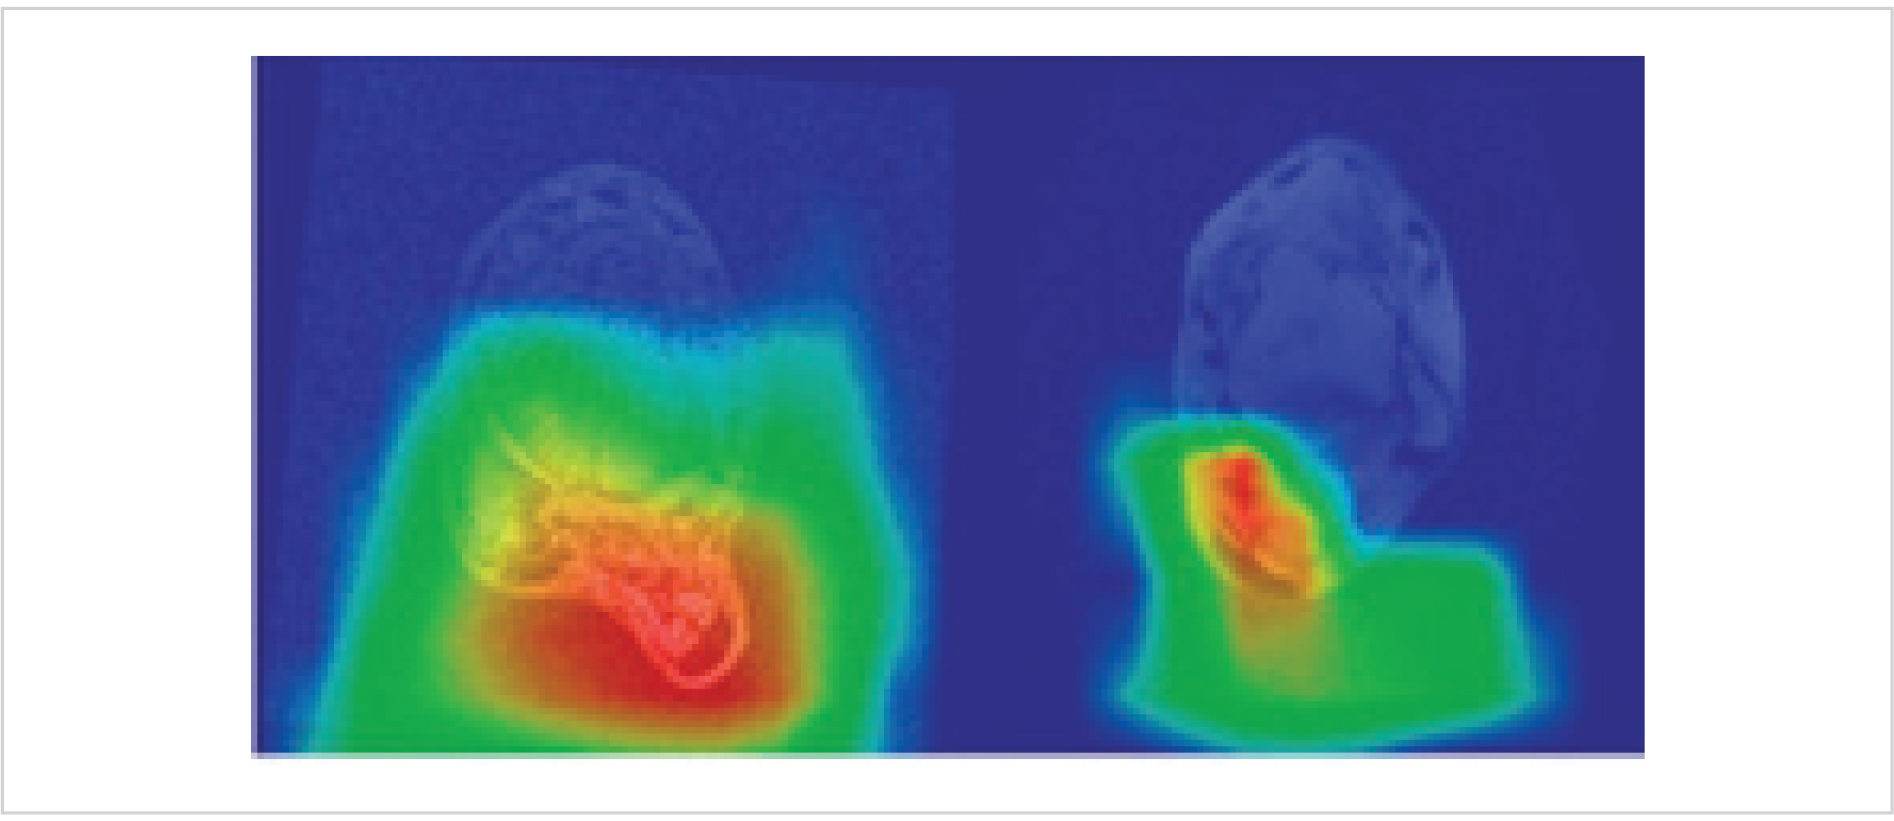
\includegraphics[width=1\textwidth]{figures/XAI.jpg}
	\caption{Analiza wizualna procesu wnioskowania sieci z zaznaczonym obszarem zainteresowania.}\label{fig:XAI}
\end{figure}
Można zaobserwować, że obszar zainteresowania wykorzystanej w eksperymentach sieci neuronowej obejmuje ROI jak i tkanki okalające. W celu zilustrowania zmian w czasie, na Rys. \ref{fig:3DXAI} pokazano izopowierzchnie przechodzące przez granicę obszaru zainteresowania w trójwymiarowych badaniach.
\begin{figure}[]
	\centering
	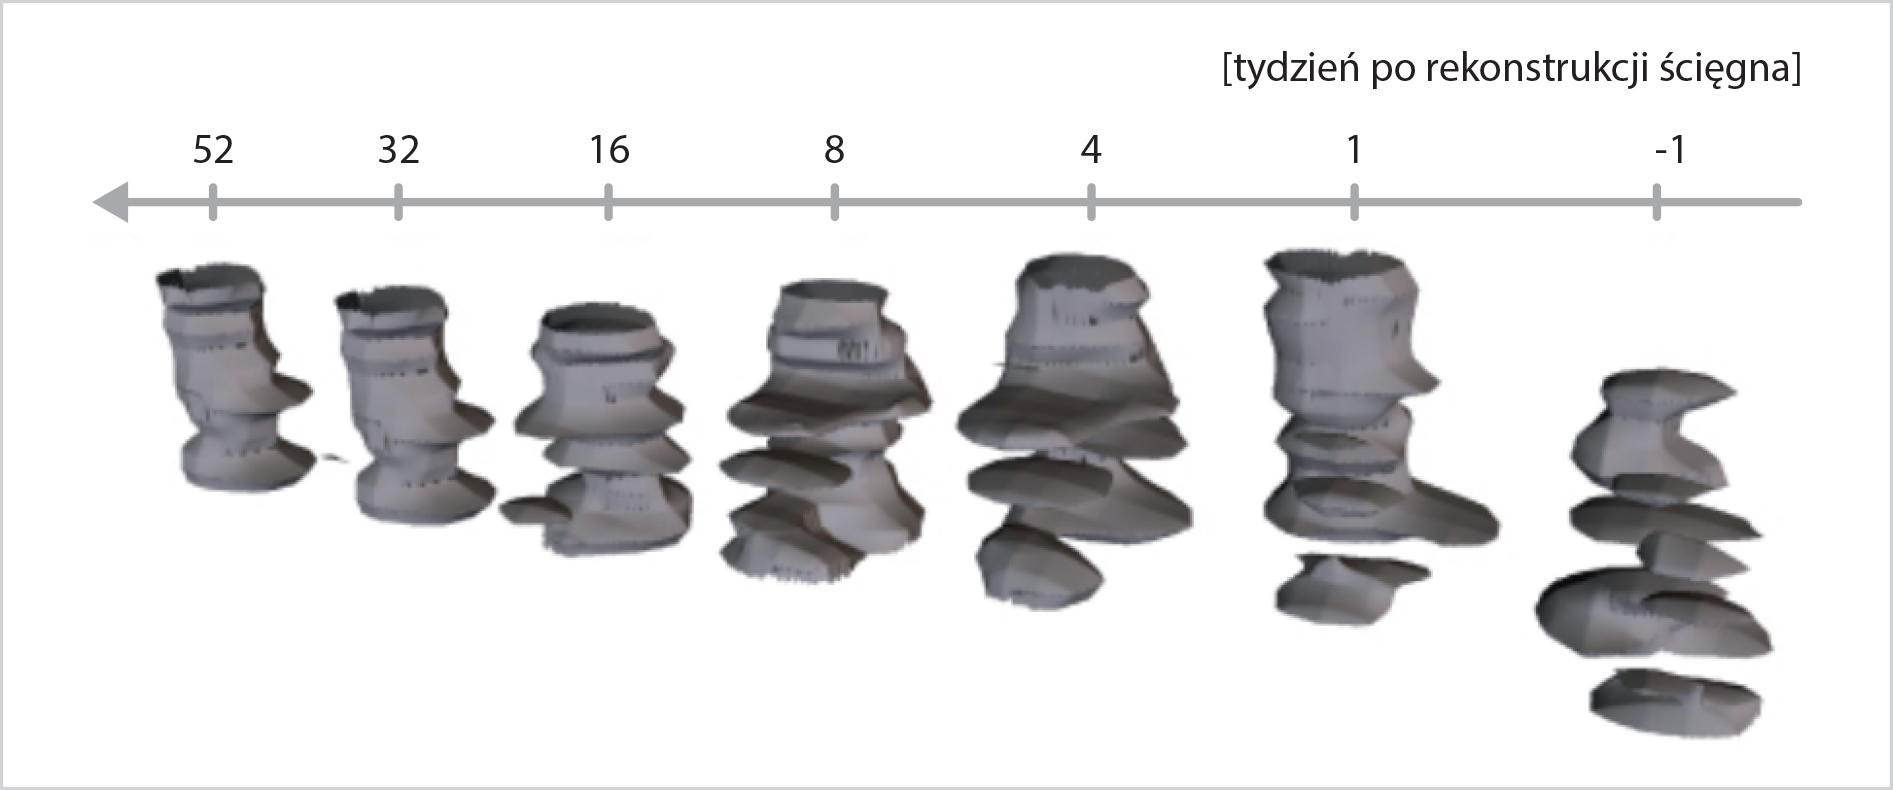
\includegraphics[width=1\textwidth]{figures/3DXAI.jpg}
	\caption{Trójwymiarowa wizualizacja zmian obszaru zainteresowania w kolejnych etapach gojenia się ścięgna.}\label{fig:3DXAI}
\end{figure}
Początkowo cechy w kolejnych przekrojach na podstawie, których wnioskuje sieć znajdują się w większym rozrzuceniu niż na końcu monitorowanego etapu gojenia się ścięgna.

Podsumowując, optymalna fuzja cech z widocznego obszaru ocenianego przez sieć neuronową oraz ROI umożliwia bardziej skuteczną ocenę całego procesu poprzez zapewnienie zgrubnej oceny z użyciem sieci i szczegółowej, z dołączenia predyktorów z ROI, bardziej odpornej na szum. 

\section{Ocena procesu gojenia}
\label{seq:valuation}
W ramach tego eksperymentu zostanie przedstawiona szczegółowa analiza wyników oceny procesu gojenia z wykorzystaniem proponowanej w tej pracy metody. \linebreak W pierwszej kolejności dokonano zgrubnej analizy. Przeanalizowano macierze błędu dla rożnych klas: (1) tygodni oceny, gdzie wartością jest średni błąd absolutny (MAE); (2) zakresu oceny (0--7), gdzie wartością jest liczba występowań. Następnie zostały przedstawione \textit{krzywe gojenia} tj. ocena zmiany w czasie poszczególnych parametrów ankiety. Porównane zostały szczegółowo, dla wszystkich testowych pacjentów, wyniki metody automatycznej z wzorcem odniesienia (ang. \textit{ground-truth}) tj. oceną eksperta radiologa.

\subsection{Macierze błędu}

Celem zdefiniowania ogólnych różnic między oceną radiologa i propozycją automatycznej metody, zestawiono dwa rodzaje macierzy błędu. W pierwszej kolejności jako klasę wybrano tydzień gojenia się ścięgna. Wyniki uzyskane z użyciem metody automatycznej porównano z oceną radiologa wykorzystując miarę średniego błędu absolutnego. Do obliczeń wykorzystano pacjentów testowych. Oddzielnie dla wszystkich 6-ciu parametrów wyznaczono macierze błędu i przedstawiono je na Rys.~\ref{fig:CM_MAE}. 

Z wykorzystaniem macierzy w stosunkowo łatwy sposób można określić w jakim stopniu wyniki ocen w poszczególnych tygodniach są do siebie zbliżone. \linebreak W przypadku możliwie najlepszego odwzorowania oceny radiologa przez nową metodę, minimalne błędy znajdowałyby się na diagonali przedstawionych wykresów. Dla poszczególnych parametrów można jednak zaobserwować dryf wartości minimalnych błędów. Pole powierzchni ($PP_d$) pomiędzy krzywą określającą wartości minimalne MAE a diagonalą zostały zebrane w Tabeli \ref{tab:dryf_meas}.
\vspace{10px} 
\begin{table*}[h!]
	\caption{Ocena dryfu krzywej łączącej minima lokalne wartości MAE w macierzach błędów z klasą przyjętą jako tydzień rehabilitacji.}
	\begin{center}
		\begin{tabular}{l||c|c|c|c|c|c}
		
			& \textbf{SCT} & \textbf{TT} & \textbf{STE} & \textbf{TE} & \textbf{TU} & \textbf{TisE}\\ 
			\hline \hline
			$PP_d$ &18&10&42&13&30&17\\	
					
		\end{tabular}
	\end{center}
	\label{tab:dryf_meas}
\end{table*}

\begin{figure}[]
	\centering
	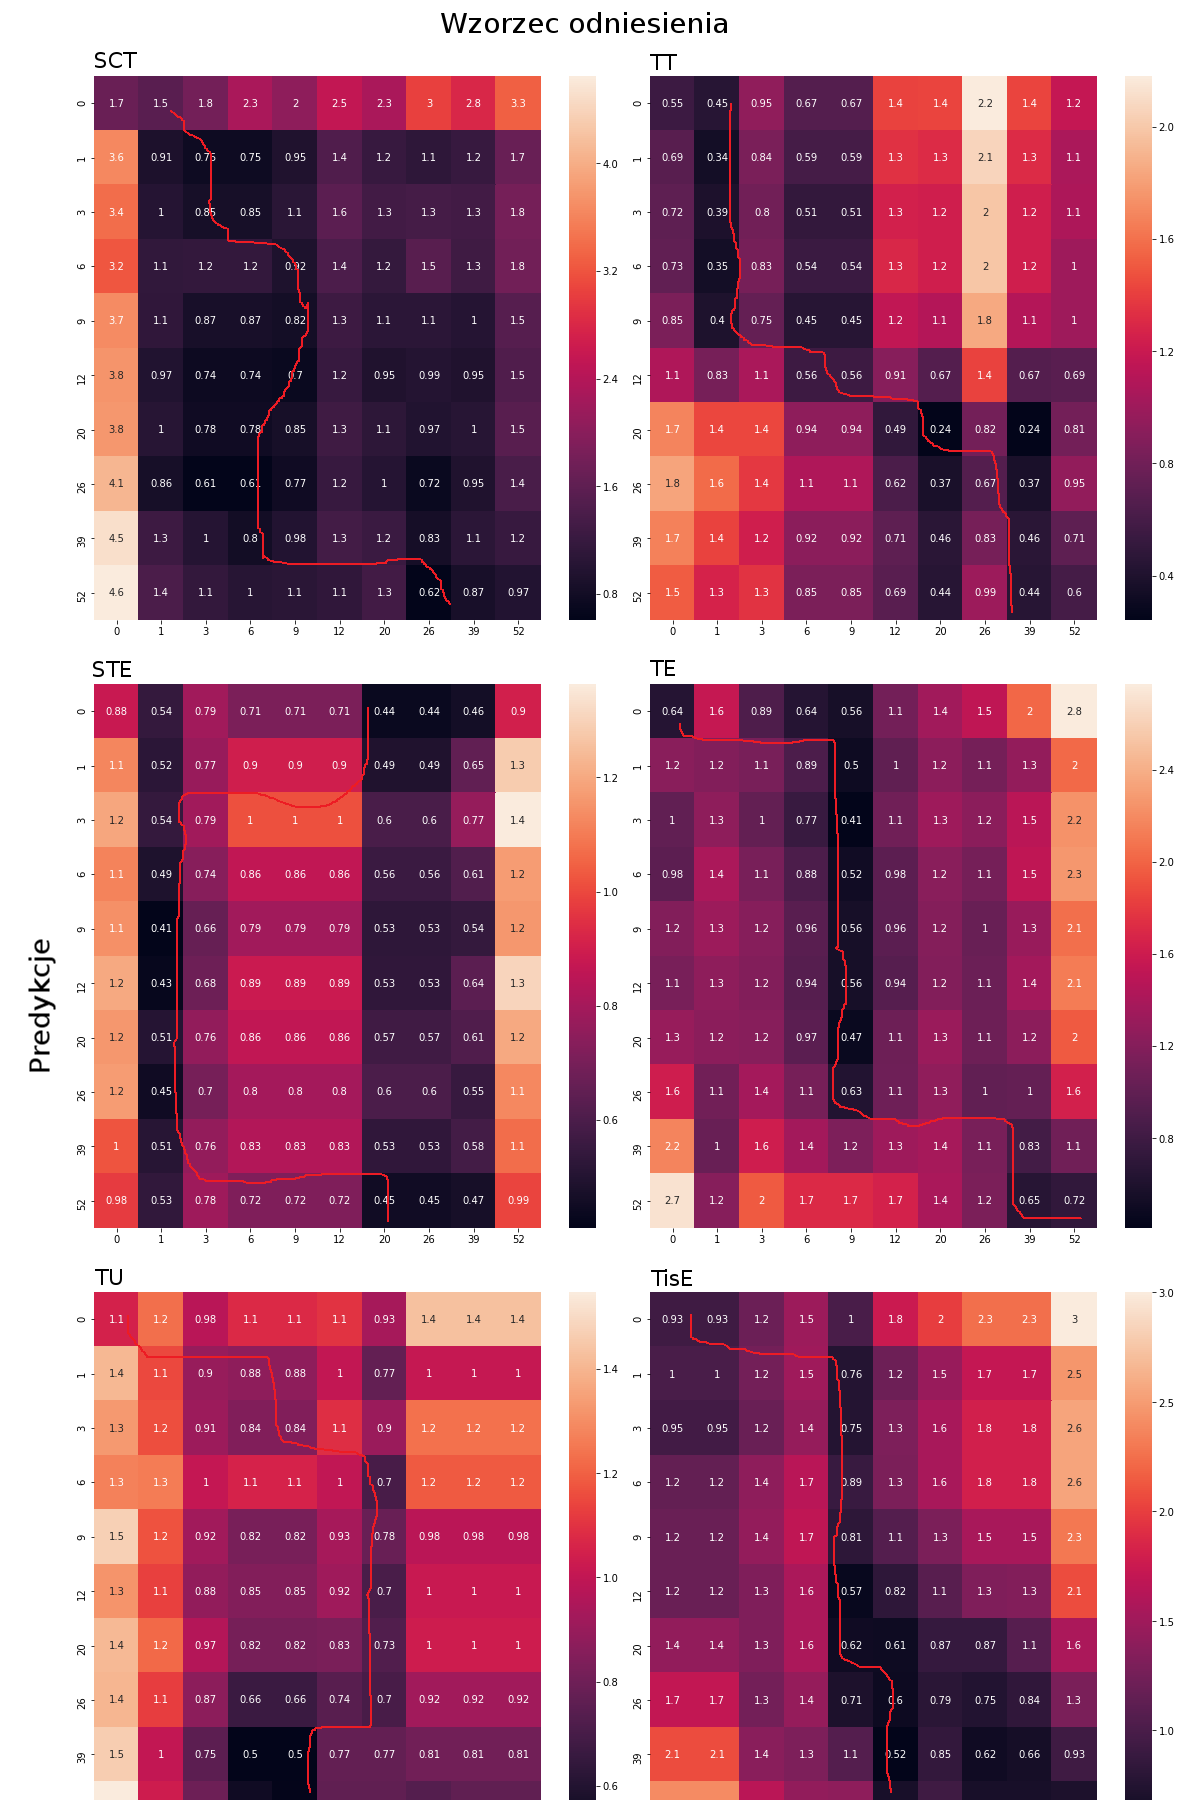
\includegraphics[width=0.9\textwidth]{figures/cm.png}
	\caption{Macierz średniego błędu absolutnego dla oceny pacjentów testowych.}\label{fig:CM_MAE}
\end{figure}
\newpage
Najlepsze rezultaty (najmniejszy $PP_d$) uzyskano dla parametru TT, a najgorszy dla STE, co oznacza, że w tych przypadkach ocena automatyczna najlepiej \linebreak i najgorzej przypomina ocenę radiologa. Kolejne, najlepsze rezultaty otrzymano dla parametrów opisujących obrzęki tj. TE i TisE oraz spójność ścięgna (SCT). Drugi najgorszy wynik został uzyskany dla parametru TU oceniającego jednorodność ścięgna w płaszczyźnie strzałkowej. Powyższe rezultaty są spójne z wnioskami \linebreak do wyników zamieszczonych w Tabeli \ref{tab:testset}, jednak szczegółowa analiza dryfu tydzień po tygodniu przedstawiono na Rys. \ref{fig:CM_MAE_SUMMARY} umożliwia dalsze wnioskowanie.

\begin{figure}[h]
	\centering
	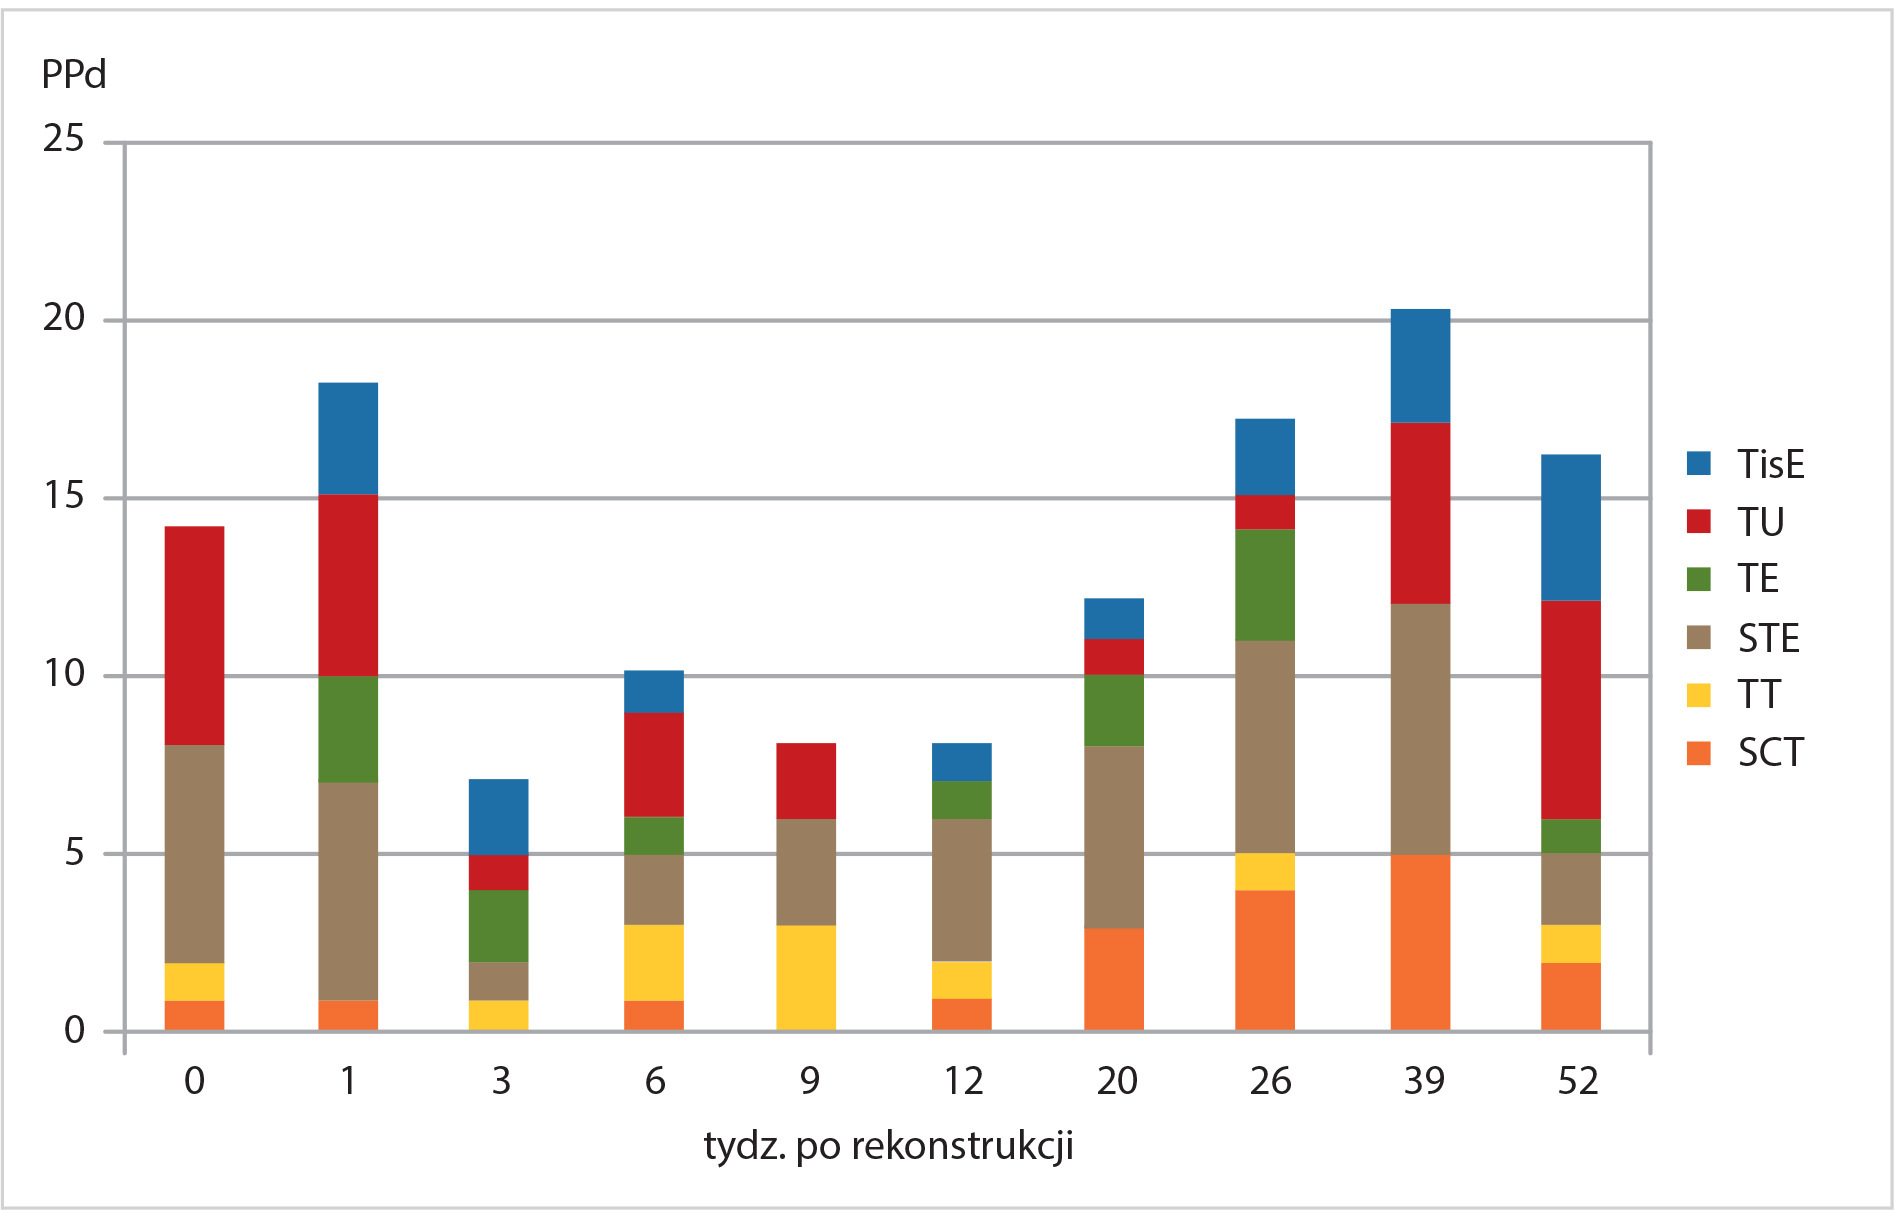
\includegraphics[width=1\textwidth]{figures/cm_summary.jpg}
	\caption{Wartości $PP_d$ dla parametrów z wzorca odniesienia.}\label{fig:CM_MAE_SUMMARY}
\end{figure}

Najmniejsze różnice w ocenie występują w trzecim tygodniu, czyli w pierwszym pomiarze po fazie zapalnej. Natomiast, wyróżniające dwie największe są obecne \linebreak w pierwszym oraz 39-tym tygodniu monitoringu, zatem w szczycie fazy zapalnej \linebreak i w momencie zaawansowania fazy przebudowy. 

Analizując poszczególne parametry od najlepszego pod względem $PP_d$: w przypadku parametru TT, największe różnice w ocenie widoczne są między 3--12 tyg., \linebreak a zatem na przełomie fazy poliferacji i przebudowy, gdzie włókna ścięgniste zaczynają się ukierunkowywać i zmienia się grubość ścięgna. Dla TE największe odchylenia zaobserwowano dla przełomu fazy zapalnej i poliferacji -- tydz. 1 oraz zaawansowanej przebudowy w 26-tym tyg. Podobny schemat zachowany jest dla TisE, \linebreak z tą różnicą, że oprócz przełomu fazy zapalnej, odchylenia są widoczne w całym okresie przebudowy. Może to świadczyć o różnicy w ocenie płynów nagromadzonych w obrzękach. W przypadku SCT, różnice w ocenie spójności włókien uwidaczniają się w fazie przebudowy, kiedy to automatyczna metoda nie wskazuje na znaczący postęp w stosunku do wyniku z 26-tego tygodnia. W przypadku dwóch parametrów uzyskujących najgorszy wynik $PP_d$ tj. TU i STE rozbieżności są widoczne \linebreak w całym okresie monitoringu, w szczególności w fazie zapalnej i przebudowy. Faza zapalna jest najbardziej dynamiczna, natomiast faza przebudowy była monitorowana w najdłuższych interwałach, co może powiększać różnice w obrazach tkanek \linebreak w obu przypadkach. 

Do dalszej analizy różnic między ocenami wykorzystano macierze błędu, gdzie klasą jest nota przyznawana w ocenie parametrów (zob. Rys. \ref{fig:cmscores}).
\begin{figure}[h]
	\centering
	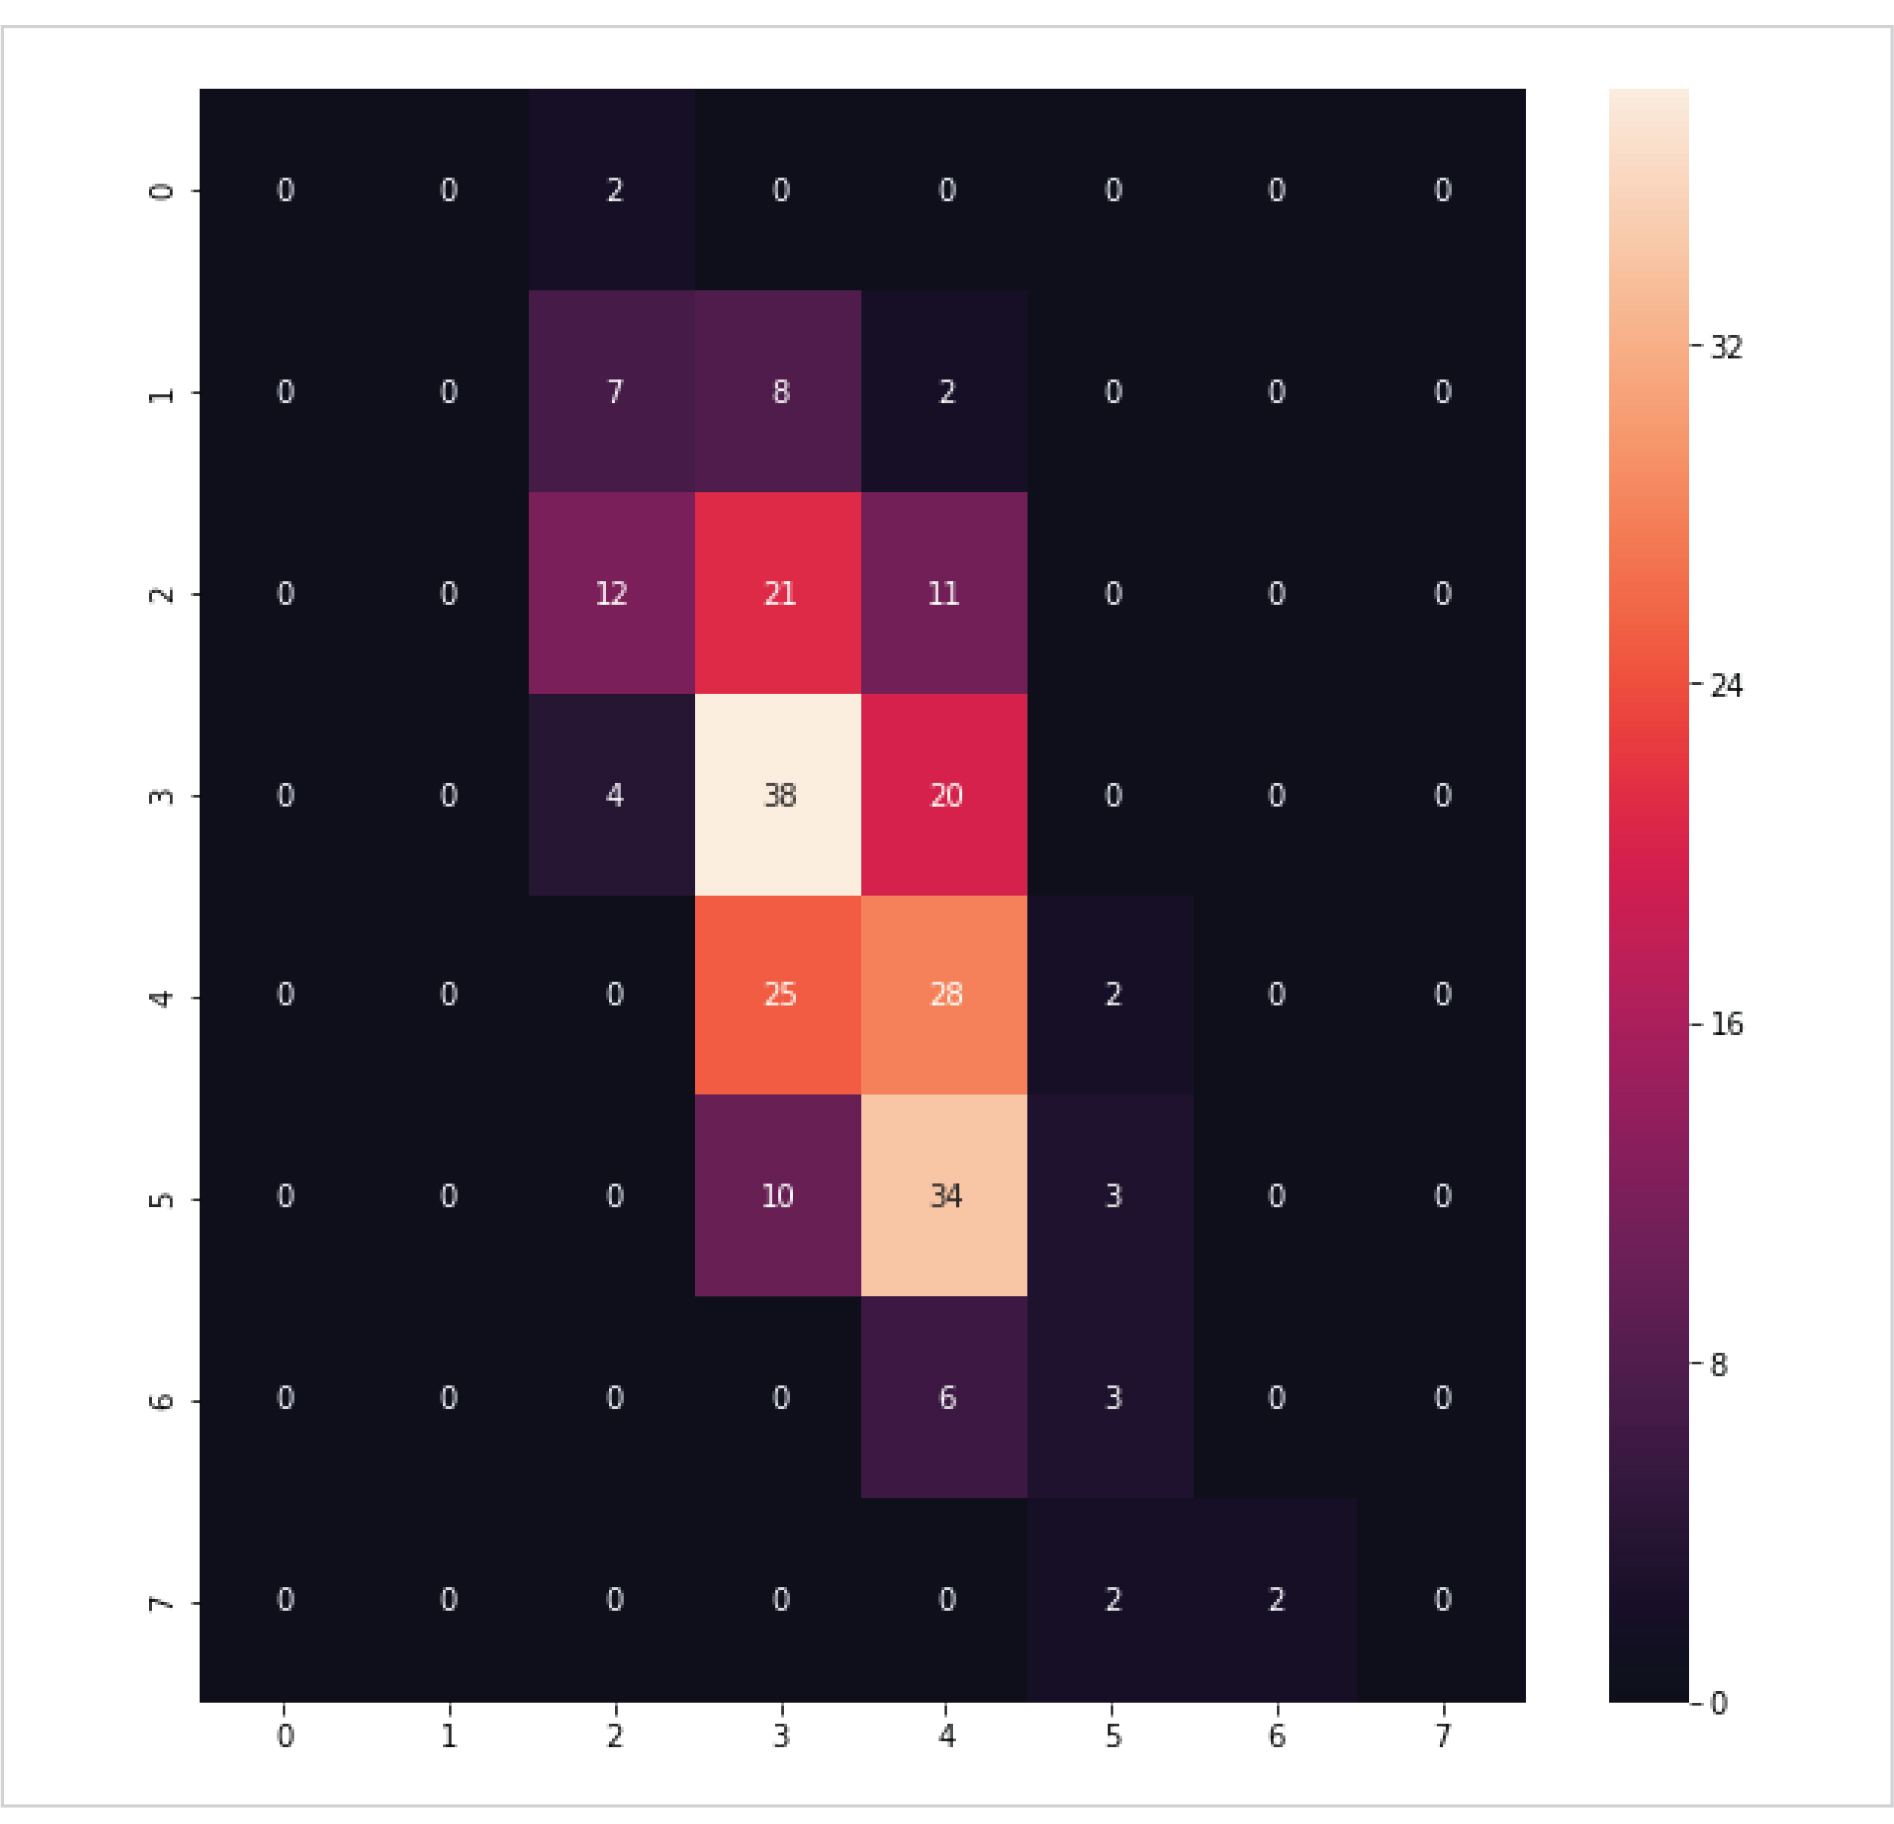
\includegraphics[width=0.9\textwidth]{figures/cmScores.jpg}
	\caption{Macierz błędu dla noty jako klasy.}\label{fig:cmscores}
\end{figure}

Największą zgodność otrzymano dla 2, 3 i 4. Notę 5 najczęściej automatyczna metoda oceniła jako 4, podobnie jak notę 6. Notę 7, dwukrotnie oceniona została jako notę 5 albo 6. W przypadku niskich wyników oceny, 1 najczęściej wystąpiła jako nota 2 (7 razy) lub 3 (8 razy). Natomiast nota 0 wystąpiła jako 2. Wartości błędów dla poszczególnych tygodniach przedstawiono na Rys. \ref{fig:cmscores_summary}.

\begin{figure}[h]
	\centering
	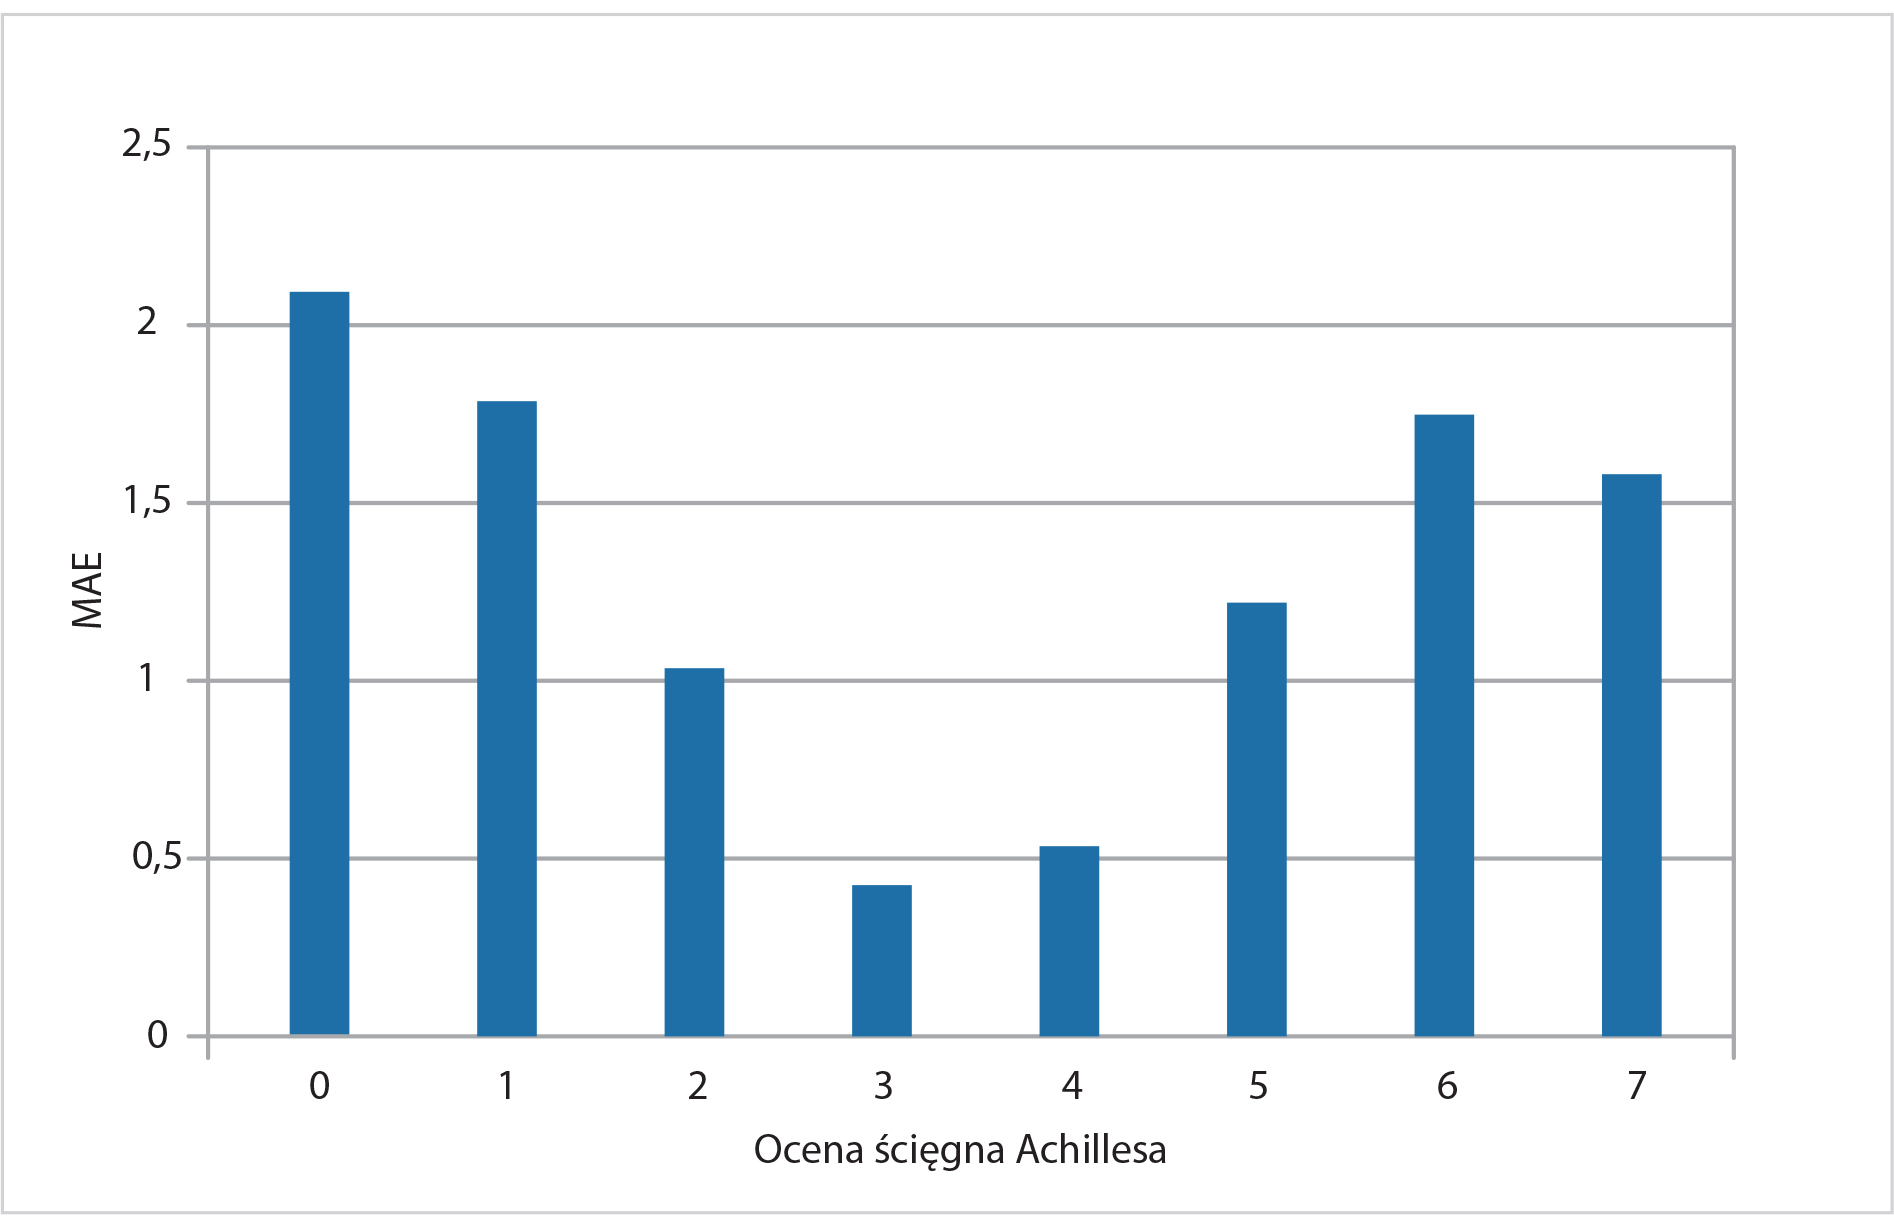
\includegraphics[width=1\textwidth]{figures/cmScores_summary.jpg}
	\caption{MAE w obrębie klas.}\label{fig:cmscores_summary}
\end{figure}

Można zaobserwować, że najmniejsze błędy ($<$1) otrzymywane są w zakresie not 2--4. Dla noty 5 wynik jest nieznacznie gorszy i osiąga poziom MAE=1,15. \linebreak W pozostałych notach skrajnych błąd wynosi $>$ 1,5. Wyniki są związane z faktem, że metoda automatyczna charakteryzuje się mniejszym zakresem oceny, co wynika z zastosowania w algorytmie meta-regresji. Wartości oceny nigdy nie osiągają not skrajnych tj. 7 lub 0--1. 

\subsection{Krzywe gojenia}
 Dla czterech pacjentów testowych, dla każdego z dziesięciu kroków czasowych, zestawiono wyniki oceny automatycznej z oceną eksperta radiologa. Na kolejnych sześciu rysunkach zaprezentowano rezultaty dla wszystkich parametrów z ankiety. Jako pierwszy przedstawiono parametr SCT (zob. Rys. \ref{fig:SCT}).
\begin{figure}[h!]
	\centering
	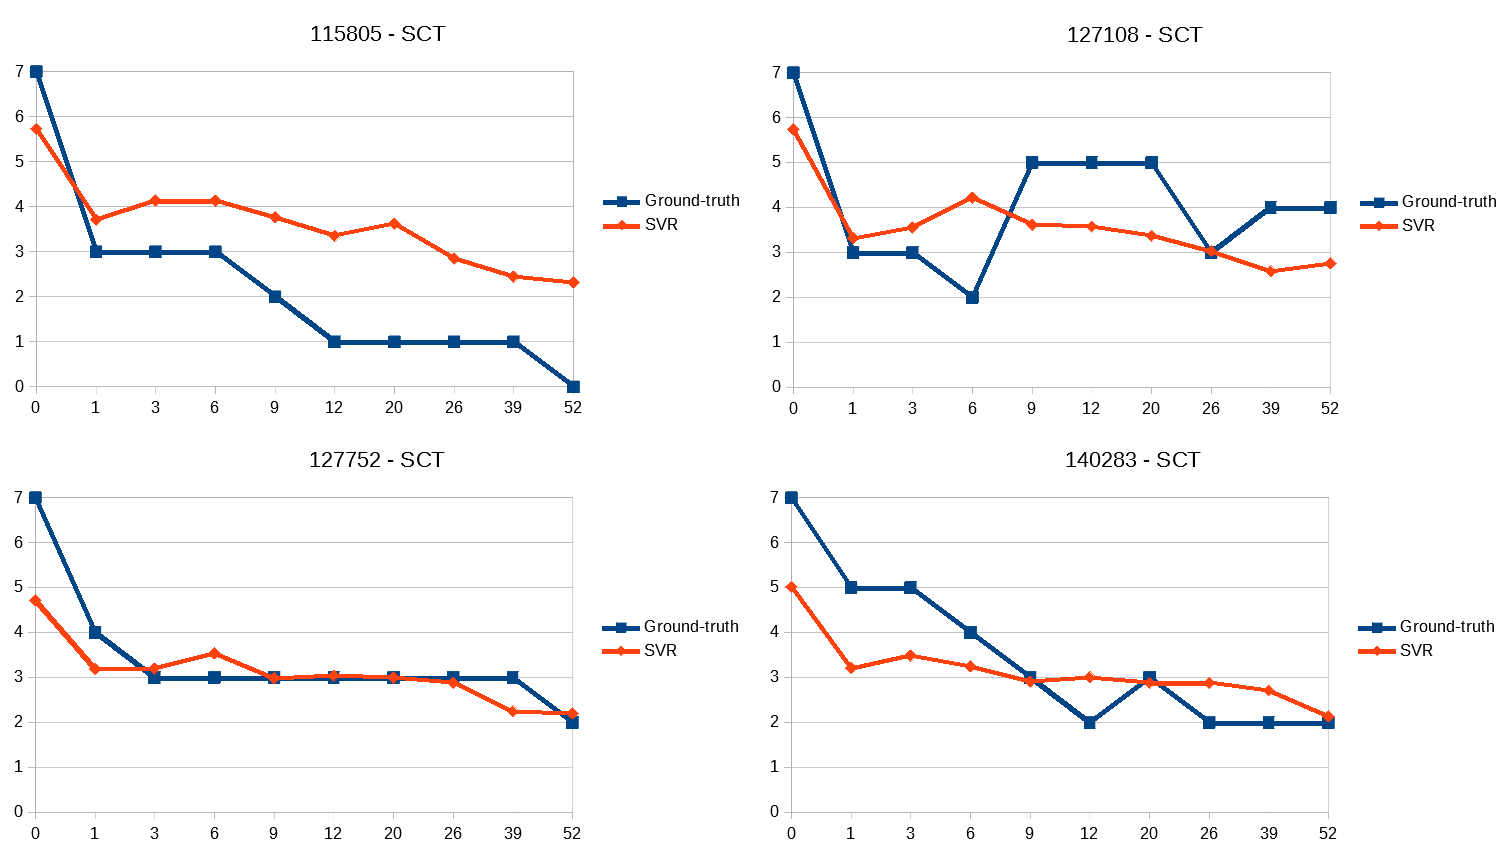
\includegraphics[width=1\textwidth]{figures/SCT.png}
	\caption{Ocena parametru SCT.}\label{fig:SCT}
\end{figure}

Zgodnie z opisem zamieszczonym w p. \ref{seq:ground-truth} dotyczy on stanu uszkodzeń śródścięgnistych wewnątrz obszaru ROI. Przed interwencją chirurgiczną ścięgno jest całkowicie zerwane, stąd w tygodniu 0, reprezentującym czas na kilka dni przed operacją, ocena radiologa wynosi 7, dla każdego z pacjentów. Po zszyciu w 3-ech z 4-ech przypadkach, proces postępuje z malejącym trendem do osiągnięcia małych, bądź braku uszkodzeń (jedyna anomalia, mogąca wynikać z omawianych wcześniej czynników zaburzających proces gojenia się, widoczna jest w 20-tym tyg. dla pacjenta 140283). W przypadku pacjenta 127108 proces gojenia się jest odmienny, przebiega z wyraźnie zmiennym trendem, jak również kończy się oceną 4, interpretowaną jako dość duże uszkodzenia. Ocena automatyczna proponowana w tej pracy przybliża trendy oceny radiologa, sugerując duże lub bardzo duże uszkodzenia na początku procesu i małe uszkodzenia w 3-ech z 4-ech przypadkach na końcu. Jedynie dla pacjenta 127108 sugerowana nota końcowa oznacza uszkodzenia średniej wielkości. Poza pojedynczym maksymalnym błędem (MAX-AE) występującym w 20-tym tyg. w ocenie pacjenta 115805, największe obserwowalne różnice w ocenie występują przed operacją. \linebreak We wszystkich czterech przypadkach ocena automatyczna stanu ekstremalnie dużych uszkodzeń związanych z całkowitym zerwaniem nie występuje, co wynika z ogólnie mniejszego zakresu punktacji metody automatycznej. 

Kolejnym analizowanym parametrem jest TT. Wykresy krzywych gojenia przedstawiono na Rys. \ref{fig:TT}.    
\begin{figure}[h!]
	\centering
	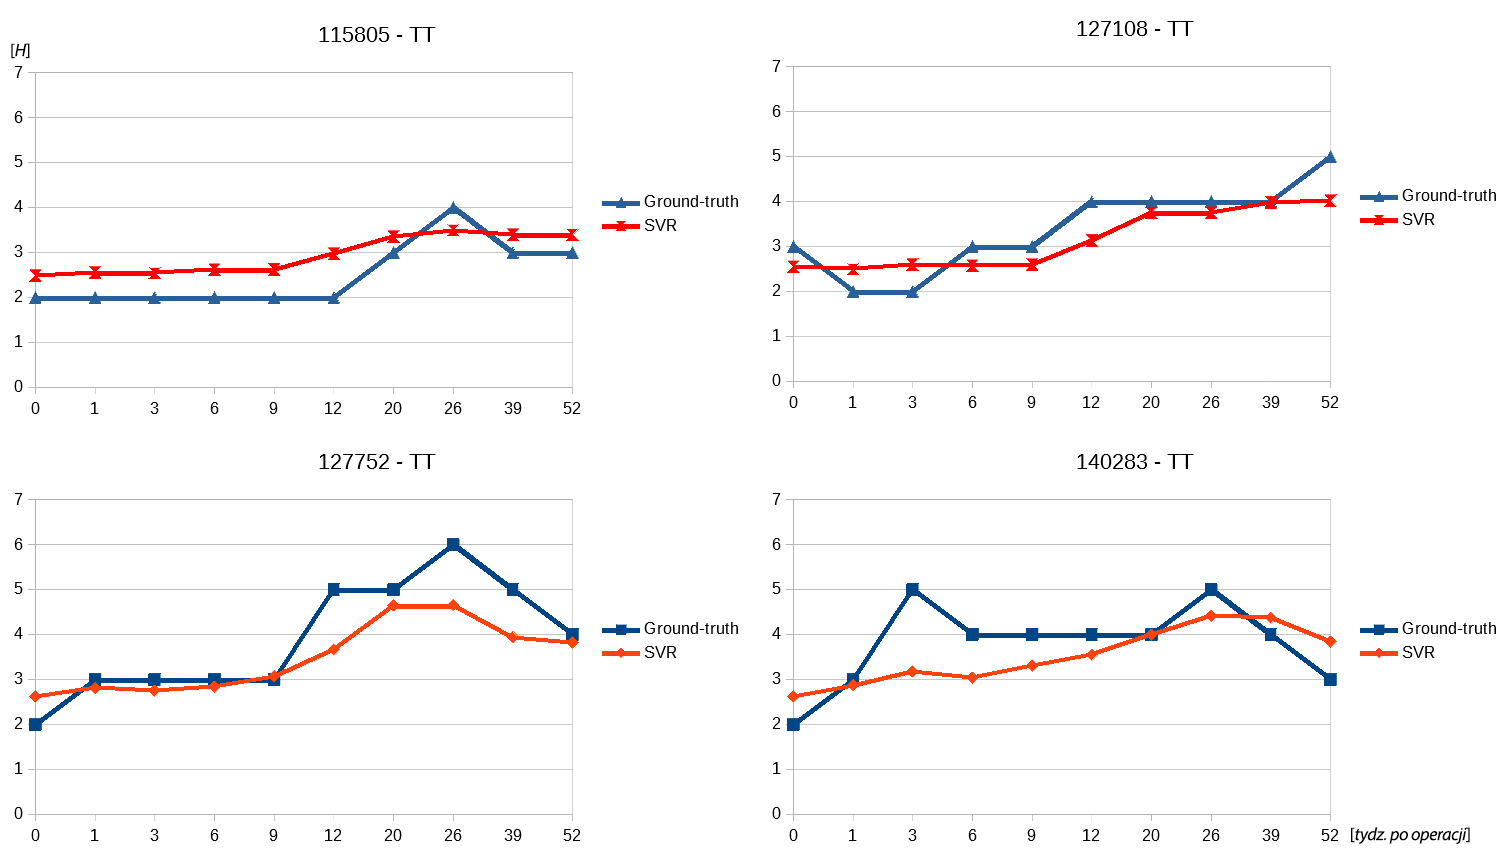
\includegraphics[width=1\textwidth]{figures/TT.png}
	\caption{Ocena parametru TT.}\label{fig:TT}
\end{figure}
Parametr ten zgodnie z przedstawioną interpretacją związany jest z oceną pogrubienia ścięgna. Na początku procesu pogrubienie jest małe lub średnie (9--12 mm.), następnie w fazie poliferacji i początkach przebudowy rośnie, co związane jest z przyrostem włókien ścięgnistych, by finalnie, w większości przypadków, ponownie zmaleć w wyniku przebudowy struktury i pozostawienia jedynie dobrze ukierunkowanych, wytrzymałych struktur. Dla pacjentów 115805 \linebreak i 127752, w ocenie radiologa proces przebiega zgodnie z wyżej przedstawionym opisem. W przypadku pacjenta 140283 widoczna jest anomalia w 3-ecim tyg., co może mieć związek z fluktuacjami np. nadmiernym obciążeniem ścięgna. Ponownie, jedynie w przypadku pacjenta 127108, gojenie przebiega odmiennie i po operacji pogrubienie rośnie, aż do 52-ego tyg. 

Błąd (MAE), równy 0,56, osiągnięty dla oceny tego parametru jest najniższy spośród wszystkich sześciu, co widoczne jest w przebiegach krzywych gojenia, które dobrze przybliżają ocenę radiologa. Anomalia w 3-ecim tyg. występująca u pacjenta 140283 nie została dobrze wykryta i w rezultacie błąd maksymalny (MAX-AE) wyniósł 1,82. W celu detekcji przyczyny konieczna jest dalsza analiza i w pierwszej kolejności weryfikacja, czy błąd popełniony został przez ocenę radiologa, czy metodę.

Następnym analizowanym parametrem jest STE. Wykresy krzywych gojenia przedstawiono na Rys. \ref{fig:STE}.
\begin{figure}[h!]
	\centering
	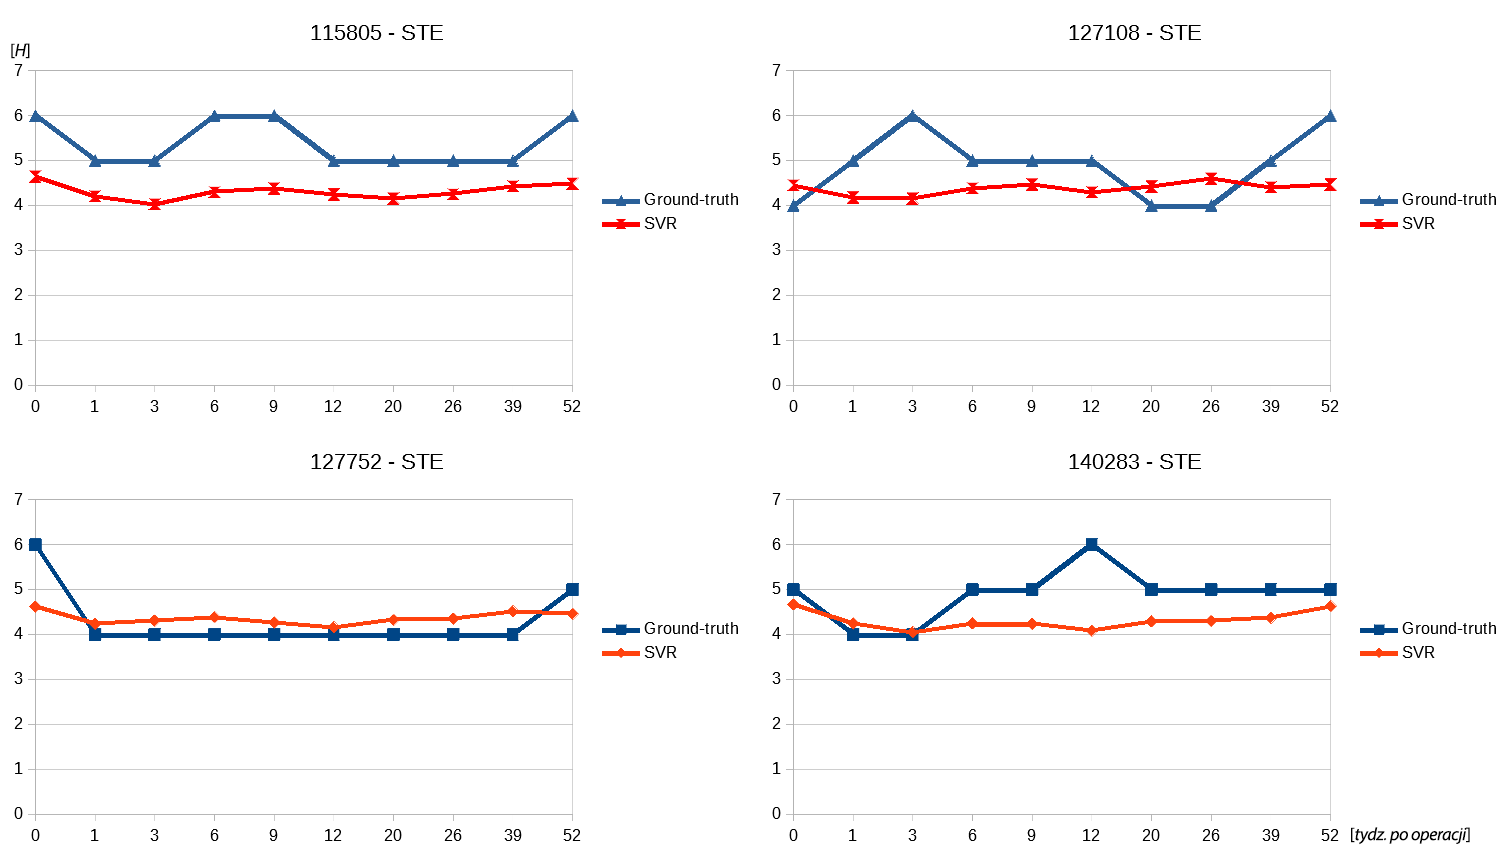
\includegraphics[width=1\textwidth]{figures/STE.png}
	\caption{Ocena parametru STE.}\label{fig:STE}
\end{figure}
Parametr ten związany jest z oceną granic pomiędzy ROI, a zewnętrznymi tkankami. Ścięgno po zerwaniu nigdy nie odzyskuje zdrowych granic, stąd ocena radiologa oscylująca w zakresie 4--6. Zakres oceny automatycznej jest jeszcze mniejszy i wynosi po zaokrągleniu 4--5. Skutkiem tak niskich zakresów jest najgorszy wynik miary Corr spośród wszystkich sześciu parametrów, co oznacza, że drobne zmiany krawędziowe nie są dobrze oceniane przez proponowaną metodę automatyczną. Z uwagi na mały zakres zmian, MAE i MAX-AE osiągnęły drugi najlepszy wynik. Na tym etapie informatywność tego parametru pozostaje wątpliwa i konieczna jest dalsza weryfikacja.

Jako czwarty parametr przedstawiono TE. Uzyskane krzywe gojenia zaprezentowano na Rys. \ref{fig:TE}.
\begin{figure}[h!]
	\centering
	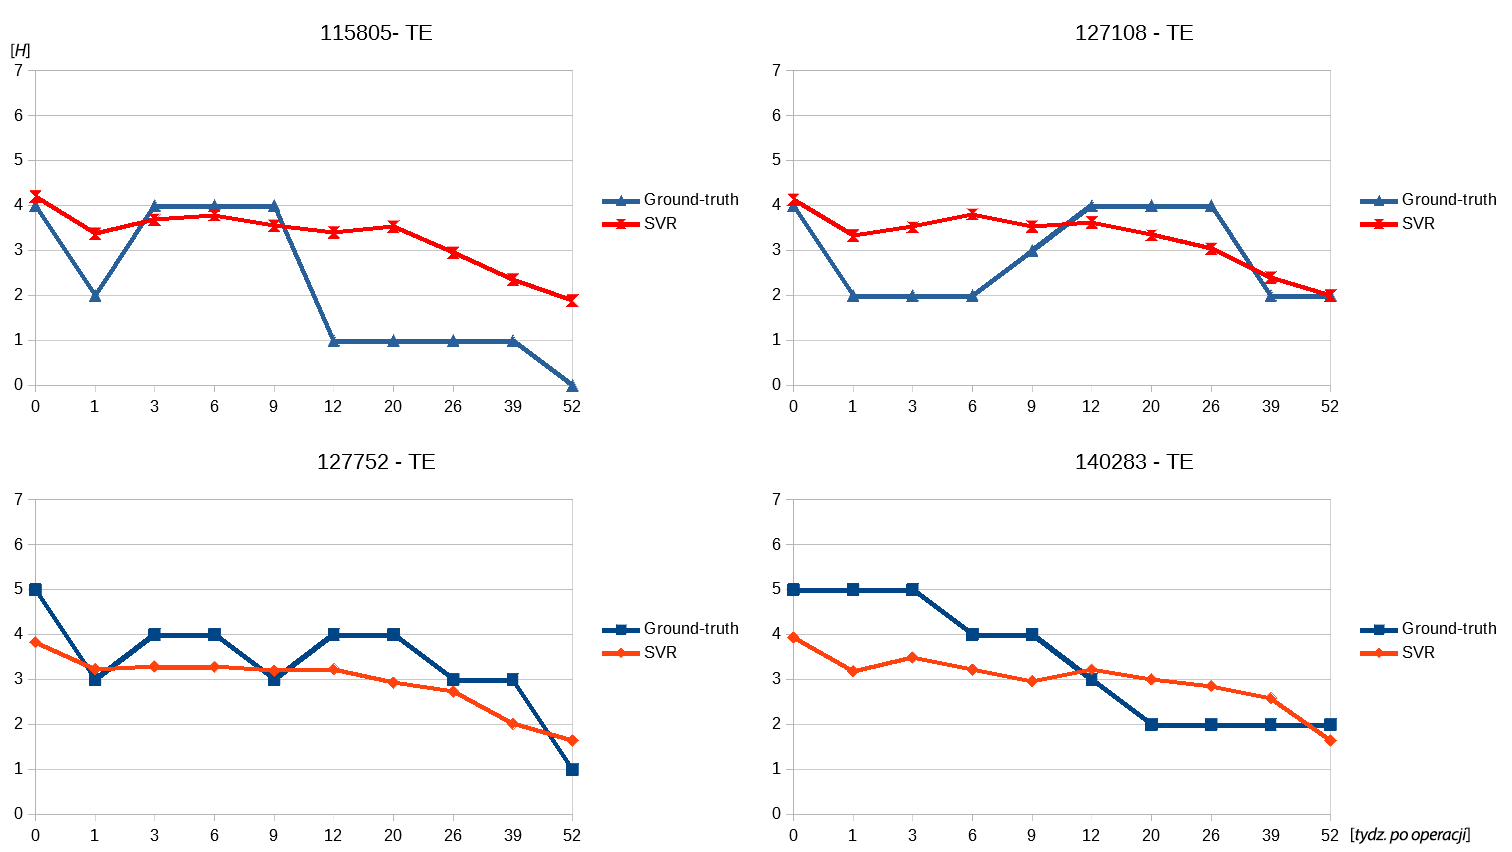
\includegraphics[width=1\textwidth]{figures/TE.png}
	\caption{Ocena parametru TE.}\label{fig:TE}
\end{figure}
W tym przypadku ocena radiologa skupiona jest na analizie płynów gromadzących się w obszarze ROI, powodujących jego obrzęk. W większości przypadków, zszycie ścięgna powoduje redukcję płynów w ROI, które następnie \linebreak w wyniku intensywnych procesów zapalnych i budowy nowych włókien ulegają ponownej akumulacji. W ostatniej fazie przebudowy, z uwagi na zmniejszenie intensywności procesów, objętość płynów ponownie jest redukowana. Dla wszystkich czterech pacjentów ocena radiologa oddaje powyższy opis. W przypadku pacjenta 127108 można zaobserwować dłuższe fazy redukcji i akumulacji płynu, co ponownie potwierdza odmienność procesu gojenia dla tego przypadku. Interesujący jest przypadek pacjenta 140283, gdzie w tygodniu 1 po operacji minimum lokalne widoczne jest tylko w wyniku oceny automatycznej. W tym przypadku rozdzielczość skali radiologa okazała się być zbyt mała. Szukając powodów błędów maksymalnych, ponownie można wskazać jako podstawowy powód mniejszy zakres zmian oceny automatycznej. W 12 tyg. oceny pacjenta 115805 występuje silna redukcja obrzęku. W ocenie automatycznej widoczne jest lokalne minimum, ale jego wartość odbiega od wzorca o 2,48, a w następnym kroku o 2,52 osiągając MAX-AE. 

Przedostatnim z analizowanych parametrów jest TU. Krzywe gojenia zostały zaprezentowane na Rys. \ref{fig:TU}.  
\begin{figure}[h!]
	\centering
	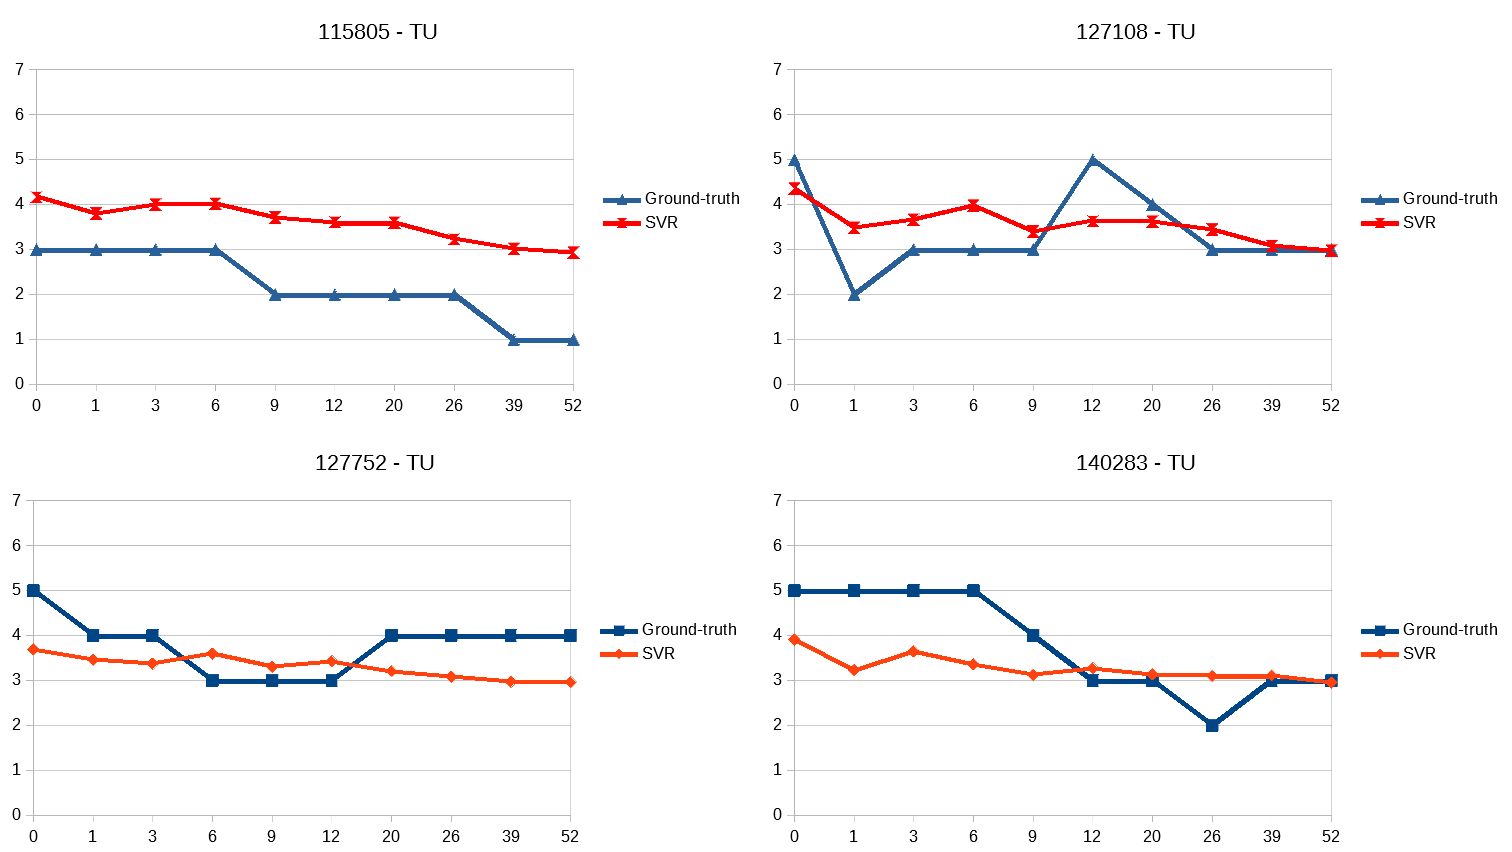
\includegraphics[width=1\textwidth]{figures/TU.png}
	\caption{Ocena parametru TU.}\label{fig:TU}
\end{figure}
Jest to jedyny parametr oceniany w całości w płaszczyźnie strzałkowej. Przy jego użyciu interpretowana jest jednorodność ścięgna widoczna w postaci charakterystycznego zdrowego warkocza włókien. Struktura \linebreak ta w procesie gojenia się ulega stopniowej poprawie, co odzwierciedlają oceny radiologa dla pacjentów 115805 i 140283 (z jedną anomalią w 26-tym tyg.). Dla pacjenta 127752 jednorodność ścięgna ulega pogorszeniu na przełomie 12-tego i 20-tego tyg., co może być wynikiem czynników zewnętrznych wpływających na przebieg gojenia. Natomiast krzywa dla pacjenta 127108 ponownie zawiera odmienne trendy, zwłaszcza na przełomie 9-tego i 12-tego tyg. Dla automatycznej oceny, parametr oceniany jest z drugim (zaraz po STE) najgorszym wynikiem pod względem Corr i również \linebreak z drugim, najgorszym MAE. Analiza automatyczna bazuje na metodzie wytrenowanej jedynie z wykorzystaniem przekrojów osiowych. Uzyskane wyniki są zatem efektem agregowanych w mierze $H$ wartości lub korelacji z innymi parametrami. 
\newpage
Jako ostatni został przeanalizowany parametr TisE. Charakteryzuje on obrzęk \linebreak w przestrzeni międzypowięziowej ścięgna Achillesa. Krzywe gojenia widoczne \linebreak są na Rys. \ref{fig:TisE}.
\begin{figure}[h!]
	\centering
	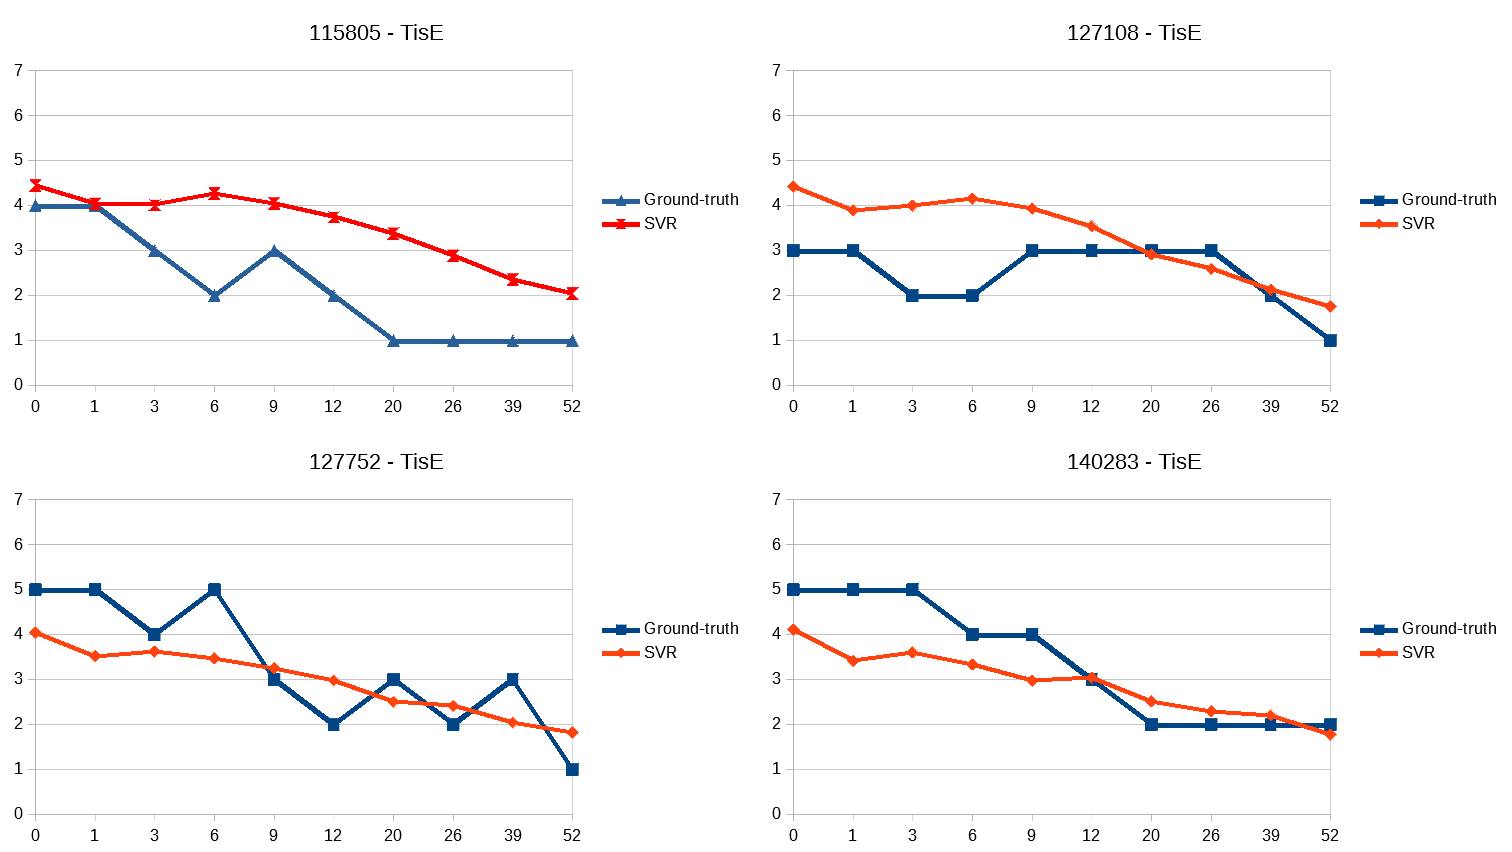
\includegraphics[width=1\textwidth]{figures/TisE.png}
	\caption{Ocena parametru TisE.}\label{fig:TisE}
\end{figure}
Jest to jedyny parametr oceniany w całości na zewnątrz ROI, tylko z wykorzystaniem cech DL. Na przełomie fazy poliferacji i remodelingu (tydz. 6--9) następuje charakterystyczny, krótkotrwały wzrost płynów w tym obszarze, wynikający z intensywności procesu. W ocenach radiologa, szczególnie widoczny jest on dla pacjenta 115805 i 127752. Dla pacjenta 140283 widoczna jest stagnacja, \linebreak a dla 127108 zwiększenie obrzęku, które utrzymuje się przez kolejne etapy do 26-tego tyg. W krzywych wygenerowanych w ocenie automatycznej widoczne są również maksima lokalne w okolicach przełomu faz gojenia się. Są one jednak przesunięte względem oceny radiologa (tydz. 3--6), co wymaga dalszej analizy.

\subsection{Ocena holistyczna}

W celu efektywnego porównania nowych zmiennych opisujących biomechanikę ścięgna i wyniku ATRS z predykcjami automatycznej metody oraz oceną radiologa, zdecydowano się również dla badań radiologicznych przeprowadzić analizę czynnikową. W obu przypadkach tj. oceny automatycznej i radiologa uzyskano minimalny udział w wyjaśnianej wariancji czynników innych niż pierwszy. Stąd możliwość wprowadzenia nowej zmiennej tj. Czynnik1 zamiast 6-ciu parametrów: SCT, STE, TE, TisE, TT, TU. Szczegółowe wyniki znajdują się w Tabeli \ref{tab:pca-gt-pred}.

\begin{table}[h]
	\centering
	\setlength{\tabcolsep}{3pt}
	\setlength\extrarowheight{2pt}
	\caption{Rezultaty analizy czynników głównych dla oceny radiologicznej i oceny automatycznej realizowanych z wykorzystaniem 6-ścio parametrycznej ankiety. Oznaczono ładunki, gdzie wartość modułu jest większa niż 0,7.}
	\label{tab:pca-gt-pred}
	\begin{tabular}{c|c|c}
		Zmienna&Czynnik1 - ocena radiologa&Czynnik1 - ocena automatyczna \\
		\hline \hline
		SCT&\textbf{-0,79}&\textbf{-0,95}\\
		\hline
		STE&0,57&\textbf{0,86}\\
		\hline
		TE&\textbf{-0,85}&\textbf{-0,94}\\
		\hline
		TisE&\textbf{-0,71}&\textbf{-0,89}\\
		\hline
		TT&\textbf{-0,76}&\textbf{-0,72}\\
		\hline
		TU&\textbf{-0,88}&\textbf{-0,94}\\
		\hline \hline	
		Udział&0,57&0,78\\
		
	\end{tabular}
\end{table}

Można zaobserwować, że udział wyjaśnianej wariancji w pierwszym czynniku jest większy dla oceny automatycznej niż dla oceny radiologa. Subiektywna ocena eksperta wprowadza nieuniknioną niepewność do pomiaru, stąd wyniki generowane przez człowieka są w większym stopniu losowe niż wyniki oceny automatycznej. 

W kolejnych badaniach zestawione zostały interkorelacje nowych zmiennych. \linebreak W Tabeli \ref{tab:gtVSpred} przedstawiono korelacje oceny automatycznej z oceną radiologa.

\vspace{10px}
\begin{table}[h]
	\centering
	\setlength{\tabcolsep}{3pt}
	\setlength\extrarowheight{2pt}
	\caption{Korelacja między oceną radiologa, a ocena automatyczną. Oznaczone wsp. korelacji są istotne z $p$ $<$ 0,05 dla $N$=30.}
	\label{tab:gtVSpred}
	\begin{tabular}{c|c|c}
		&Ocena automatyczna &Ocena radiologa \\
		\hline \hline
		Ocena automatyczna&1,0000&\textbf{0,8070}\\
		\hline
		Ocena radiologa&\textbf{0,8070}&1,0000\\
		
	\end{tabular}
\end{table}

Naturalnie, nowa zmienna opisująca ocenę radiologa koreluje z nową zmienną opisującą ocenę automatyczną. Fakt ten jest kolejnym potwierdzeniem na silny związek między zastosowanymi metodami przetwarzania obrazów i eksperckimi, ludzkimi spostrzeżeniami.
